\documentclass[12pt]{article} % Prepara un documento con un font grande
\usepackage[italian]{babel} % Adatta LaTeX alle convenzioni tipografiche italiane,
							% e ridefinisce alcuni titoli in italiano, come "Capitolo" al posto di "Chapter",
							% se il documento è in italiano

\usepackage[utf8]{inputenc} % Consente l'uso caratteri accentati italiani
\usepackage{graphicx}		% Per le immagini
\usepackage[top=2in, bottom=1.5in, left=0.5in, right=0.5in]{geometry}
\usepackage{float}
\usepackage{gnuplot-lua-tikz}

\nonstopmode

\title {Relazione di Laboratorio - Guidovia}
\author{Francesco Forcher\\
Matricola: \texttt{1073458}\\
\texttt{mailto:francesco.forcher@studenti.unipd.it}\\
\and
Francesca Damiani\\ 
Matricola: \texttt{1071072}\\
\texttt{mailto:francesca.damiani@studenti.unipd.it}\\
\and
Andrea Piccinin\\ 
Matricola: \texttt{1070620}\\
\texttt{mailto:andrea.piccinin1@studenti.unipd.it}\\
}

\date{\today}


\pagestyle{headings}
\DeclareGraphicsExtensions{.svg, .pdf, .png, .jpg} % Se due immagini hanno lo stesso nome sceglile secondo l'ordine di filetype qui

\graphicspath{ {../Gnuplot/immagini/} }%%%%%%%%%%%%%%%%%%%%%%%%%%%%%%%%EDITARE PATH!!%%%%%%%%%%%%%%%%%%%%%%%%%%%%%%%%%%%%%%%%% % Path delle immagini 















% PROVA MODIFICA DA BROWSER!!!!
%////////////////////////////////////////////////////////////////////////////////////////////////////////////////////////////
%////////////////////////////////////////////////////////////////////////////////////////////////////////////////////////////
% Fine dei dati iniziali per il latex: il documento finale inizierà da qui
\begin{document}


\maketitle % Produce il titolo a partire dai comandi \title, \author e \date
\newpage
\tableofcontents % Prepara l'indice generale



        
\newpage
\section{Obiettivi}
	Stimare il valore dell'accelerazione di gravità \textbf{g} attraverso la misurazione dell'accelerazione della slitta su un piano 
	inclinato, tenendo conto, nella seconda parte dell'esperienza, anche del contributo dell'attrito dell'aria.

\section{Descrizione dell'apparato strumentale}
	Slitta in plexiglass che, inizialmente bloccata da un elettromagnete, scorre lungo una guidovia di acciaio, il cui attrito con la slitta è rimosso da un cuscino d'aria. 
	Traguardi mobili a sensori infrarossi, collegati ad un cronometro di sensibilità \(10^{-3}\) s.
	Nella seconda parte dell'esperienza , essendo la guida posta orizzontalmente, la slitta è stata fatta muovere attraverso un impulso elettrico dato dall'elettromagnete, che ne determina la velocità iniziale. 
	

\section{Metodologia di misura}
	Nella prima parte dell'esperienza, l'elettromagnete che trattiene la slitta viene disattivato tramite un pulsante. La slitta inizia così a scorrere lungo la guidovia su cui sono posizionati i traguardi, che inviano al cronometro il tempo di percorrenza 		dell'intervallo stabilito. Le misure vengono prese partendo da 40 cm dall'elettromagnete, aumentando l'ampiezza dell'intervallo da 10 		cm a 70 cm. Le misure vengono poi ripetute applicando un disco di ottone sulla slitta in modo da modificarne il peso.
	Nella seconda parte dell'esperienza, essendo la guidovia orizzontale, si fa muovere la slitta attraverso un impulso elettrico, che ne determina la velocità iniziale. In questo caso le misure vengono prese su intervalli di 20 cm, sempre partendo da 40 cm di distanza 		dall'elettromagnete, in modo da stimare una riduzione della velocità dovuta alla forza di attrito. La velocità iniziale viene poi 		modificata interponendo tra la slitta e l'elettromagnete uno spessore in alluminio.


\newpage
\section{Presentazione dati sperimentali}	
	Riportiamo in seguito le misure tabulate, con relative statistiche.
	\subsection {Inclinazione 15', senza peso}
		La quarta misura nell'intervallo 40-60 cm ha un valore non compatibile con gli altri. Potrebbe esserci stato un errore durante la misurazione. 
		Ma adottando il modello di selezione dei dati oggettivo dei 3 sigma, poichè il valore rientra nei limiti, è
		stato lasciato.
		\begin{table}[H]
		%\caption{}
			\begin{tabular}{|l|r|r|r|r|r|r|r|}
			\hline
			Intervalli (cm) & \multicolumn{1}{c|}{40 – 50} & \multicolumn{1}{c|}{40 – 60} & \multicolumn{1}{c|}{40 – 70} & \multicolumn{1}{c|}{40 – 80 } & \multicolumn{1}{c|}{40 – 90} & \multicolumn{1}{c|}{40 – 100} & \multicolumn{1}{c|}{40 – 110} \\ \hline
			 & \multicolumn{ 7}{l|}{} \\ \hline
			\multicolumn{ 1}{|c|}{Misure (s)} & 0.648 & 1.200 & 1.714 & 2.174 & 2.594 & 2.988 & 3.348 \\ \cline{ 2- 8}
			\multicolumn{ 1}{|l|}{} & 0.644 & 1.206 & 1.701 & 2.157 & 2.582 & 2.992 & 3.384 \\ \cline{ 2- 8}
			\multicolumn{ 1}{|l|}{} & 0.642 & 1.198 & 1.700 & 2.170 & 2.578 & 2.978 & 3.380 \\ \cline{ 2- 8}
			\multicolumn{ 1}{|l|}{} & 0.639 & 1.804 & 1.706 & 2.157 & 2.586 & 2.976 & 3.354 \\ \cline{ 2- 8}
			\multicolumn{ 1}{|l|}{} & 0.644 & 1.200 & 1.697 & 2.162 & 2.588 & 2.980 & 3.361 \\ \hline
			 & \multicolumn{ 7}{c|}{} \\ \hline
			Media (s) & 0.643 & 1.3 & 1.704 & 2.164 & 2.586 & 2.983 & 3.365 \\ \hline
			Varianza del campione (s^2) & 0.001 & 0.05 & 0.001 & 0.001 & 0.001 & 0.001 & 0.001 \\ \hline
			Deviazione standard campione (s) & 0.003 & 0.2 & 0.006 & 0.007 & 0.005 & 0.006 & 0.01 \\ \hline
			Varianza della popolazione (s^2) & 0.001 & 0.07 & 0.001 & 0.001 & 0.001 & 0.001 & 0.001 \\ \hline
			Deviazione standard popolazione (s) & 0.003 & 0.3 & 0.007 & 0.008 & 0.006 & 0.007 & 0.02 \\ \hline
			Errore della media (s) & 0.001 & 0.1 & 0.003 & 0.003 & 0.003 & 0.003 & 0.007 \\ \hline
			Massimo (s) & 0.648 & 1.8 & 1.714 & 2.174 & 2.594 & 2.992 & 3.384 \\ \hline
			Minimo (s) & 0.639 & 1.1 & 1.697 & 2.157 & 2.578 & 2.976 & 3.348 \\ \hline
			\end{tabular}
		\label{15n}
		\end{table}

	\subsection {Inclinazione 30', senza peso}
		\begin{table}[H]
			\begin{tabular}{|l|r|r|r|r|r|r|r|}
			\hline
			Intervalli (cm) & \multicolumn{1}{c|}{40 – 50} & \multicolumn{1}{c|}{40 – 60} & \multicolumn{1}{c|}{40 – 70} & \multicolumn{1}{c|}{40 – 80 } & \multicolumn{1}{c|}{40 – 90} & \multicolumn{1}{c|}{40 – 100} & \multicolumn{1}{c|}{40 – 110} \\ \hline
			 & \multicolumn{ 7}{l|}{} \\ \hline
			\multicolumn{ 1}{|c|}{Misure (s)} & 0.453 & 0.848 & 1.196 & 1.514 & 1.819 & 2.088 & 2.350 \\ \cline{ 2- 8}
			\multicolumn{ 1}{|l|}{} & 0.452 & 0.846 & 1.200 & 1.518 & 1.822 & 2.093 & 2.350 \\ \cline{ 2- 8}
			\multicolumn{ 1}{|l|}{} & 0.454 & 0.850 & 1.196 & 1.520 & 1.812 & 2.093 & 2.346 \\ \cline{ 2- 8}
			\multicolumn{ 1}{|l|}{} & 0.452 & 0.849 & 1.196 & 1.522 & 1.812 & 2.092 & 2.350 \\ \cline{ 2- 8}
			\multicolumn{ 1}{|l|}{} & 0.452 & 0.846 & 1.192 & 1.514 & 1.811 & 2.099 & 2.354 \\ \hline
			 & \multicolumn{ 7}{c|}{} \\ \hline
			Media (s) & 0.453 & 0.848 & 1.196 & 1.518 & 1.815 & 2.093 & 2.350 \\ \hline
			Varianza del campione (s^2) & 0.001 & 0.001 & 0.001 & 0.001 & 0.001 & 0.001 & 0.001 \\ \hline
			Deviazione standard campione (s) & 0.001 & 0.002 & 0.003 & 0.003 & 0.004 & 0.004 & 0.003 \\ \hline
			Varianza della popolazione (s^2) & 0.001 & 0.001 & 0.001 & 0.001 & 0.001 & 0.001 & 0.001 \\ \hline
			Deviazione standard popolazione (s) & 0.001 & 0.002 & 0.003 & 0.004 & 0.005 & 0.004 & 0.003 \\ \hline
			Errore della media (s) & 0.001 & 0.001 & 0.001 & 0.002 & 0.002 & 0.002 & 0.001 \\ \hline
			Massimo (s) & 0.454 & 0.850 & 1.200 & 1.522 & 1.822 & 2.099 & 2.354 \\ \hline
			Minimo (s) & 0.452 & 0.846 & 1.192 & 1.514 & 1.811 & 2.088 & 2.346 \\ \hline
			\end{tabular}
		\label{30n}
		\end{table}

	\subsection {Inclinazione 45', senza peso}
		\begin{table}[H]
			\begin{tabular}{|l|r|r|r|r|r|r|r|}
			\hline
			Intervalli (cm) & \multicolumn{1}{c|}{40 – 50} & \multicolumn{1}{c|}{40 – 60} & \multicolumn{1}{c|}{40 – 70} & \multicolumn{1}{c|}{40 – 80 } & \multicolumn{1}{c|}{40 – 90} & \multicolumn{1}{c|}{40 – 100} & \multicolumn{1}{c|}{40 – 110} \\ \hline
			 & \multicolumn{ 7}{l|}{} \\ \hline
			\multicolumn{ 1}{|c|}{Misure (s)} & 0.367 & 0.688 & 0.974 & 1.236 & 1.477 & 1.704 & 1.908 \\ \cline{ 2- 8}
			\multicolumn{ 1}{|l|}{} & 0.368 & 0.687 & 0.972 & 1.235 & 1.478 & 1.702 & 1.912 \\ \cline{ 2- 8}
			\multicolumn{ 1}{|l|}{} & 0.367 & 0.687 & 0.974 & 1.235 & 1.470 & 1.703 & 1.906 \\ \cline{ 2- 8}
			\multicolumn{ 1}{|l|}{} & 0.368 & 0.690 & 0.974 & 1.234 & 1.480 & 1.702 & 1.910 \\ \cline{ 2- 8}
			\multicolumn{ 1}{|l|}{} & 0.368 & 0.688 & 0.973 & 1.235 & 1.481 & 1.700 & 1.912 \\ \hline
			 & \multicolumn{ 7}{c|}{} \\ \hline
			Media (s) & 0.368 & 0.688 & 0.973 & 1.235 & 1.477 & 1.702 & 1.910 \\ \hline
			Varianza del campione (s^2) & 0.001 & 0.001 & 0.001 & 0.001 & 0.001 & 0.001 & 0.001 \\ \hline
			Deviazione standard campione (s) & 0.001 & 0.001 & 0.001 & 0.001 & 0.004 & 0.001 & 0.002 \\ \hline
			Varianza della popolazione (s^2) & 0.001 & 0.001 & 0.001 & 0.001 & 0.001 & 0.001 & 0.001 \\ \hline
			Deviazione standard popolazione (s) & 0.001 & 0.001 & 0.001 & 0.001 & 0.004 & 0.001 & 0.003 \\ \hline
			Errore della media (s) & 0.000 & 0.001 & 0.001 & 0.001 & 0.002 & 0.001 & 0.001 \\ \hline
			Massimo (s) & 0.368 & 0.690 & 0.974 & 1.236 & 1.481 & 1.704 & 1.912 \\ \hline
			Minimo (s) & 0.367 & 0.687 & 0.972 & 1.234 & 1.470 & 1.700 & 1.906 \\ \hline
			\end{tabular}

		\label{45n}
		\end{table}
		
	\subsection {Inclinazione 45', con peso}
		\begin{table}[H]
			\begin{tabular}{|l|r|r|r|r|r|r|r|}
			\hline
			Intervalli (cm) & \multicolumn{1}{c|}{40 – 50} & \multicolumn{1}{c|}{40 – 60} & \multicolumn{1}{c|}{40 – 70} & \multicolumn{1}{c|}{40 – 80 } & \multicolumn{1}{c|}{40 – 90} & \multicolumn{1}{c|}{40 – 100} & \multicolumn{1}{c|}{40 – 110} \\ \hline
			 & \multicolumn{ 7}{l|}{} \\ \hline
			\multicolumn{ 1}{|c|}{Misure (s)} & 0.367 & 0.688 & 0.975 & 1.234 & 1.435 & 1.702 & 1.912 \\ \cline{ 2- 8}
			\multicolumn{ 1}{|l|}{} & 0.368 & 0.688 & 0.976 & 1.236 & 1.474 & 1.700 & 1.912 \\ \cline{ 2- 8}
			\multicolumn{ 1}{|l|}{} & 0.368 & 0.690 & 0.975 & 1.234 & 1.474 & 1.700 & 1.912 \\ \cline{ 2- 8}
			\multicolumn{ 1}{|l|}{} & 0.368 & 0.690 & 0.974 & 1.234 & 1.474 & 1.700 & 1.913 \\ \cline{ 2- 8}
			\multicolumn{ 1}{|l|}{} & 0.368 & 0.690 & 0.974 & 1.234 & 1.476 & 1.700 & 1.914 \\ \hline
			 & \multicolumn{ 7}{c|}{} \\ \hline
			Media (s) & 0.368 & 0.689 & 0.975 & 1.234 & 1.467 & 1.700 & 1.913 \\ \hline
			Varianza del campione (s^2) & 0.001 & 0.001 & 0.001 & 0.001 & 0.001 & 0.001 & 0.001 \\ \hline
			Deviazione standard campione (s) & 0.001 & 0.001 & 0.001 & 0.001 & 0.02 & 0.001 & 0.001 \\ \hline
			Varianza della popolazione (s^2) & 0.001 & 0.001 & 0.001 & 0.001 & 0.001 & 0.001 & 0.001 \\ \hline
			Deviazione standard popolazione (s) & 0.001 & 0.001 & 0.001 & 0.001 & 0.02 & 0.001 & 0.001 \\ \hline
			Errore della media (s) & 0.001 & 0.001 & 0.001 & 0.001 & 0.008 & 0.001 & 0.001 \\ \hline
			Massimo (s) & 0.368 & 0.690 & 0.976 & 1.236 & 1.476 & 1.702 & 1.914 \\ \hline
			Minimo (s) & 0.367 & 0.688 & 0.974 & 1.234 & 1.435 & 1.700 & 1.912 \\ \hline
			\end{tabular}

		\label{45p}
		\end{table}
		
	\subsection {Inclinazione 0', senza peso, senza spessore}
		\begin{table}[H]
		\begin{tabular}{|l|r|r|r|r|r|r|}
		\hline
		Intervalli (cm) & \multicolumn{1}{c|}{40 – 60} & \multicolumn{1}{c|}{50 – 70} & \multicolumn{1}{c|}{60 – 80} & \multicolumn{1}{c|}{70 – 90} & \multicolumn{1}{c|}{80 – 100} & \multicolumn{1}{c|}{90 – 110} \\ \hline
		 & \multicolumn{ 6}{l|}{} \\ \hline
		\multicolumn{ 1}{|c|}{Misure (s)} & 1.168 & 1.182 & 1.187 & 1.194 & 1.207 & 1.160 \\ \cline{ 2- 7}
		\multicolumn{ 1}{|l|}{} & 1.154 & 1.160 & 1.188 & 1.186 & 1.184 & 1.174 \\ \cline{ 2- 7}
		\multicolumn{ 1}{|l|}{} & 1.158 & 1.172 & 1.187 & 1.196 & 1.192 & 1.168 \\ \cline{ 2- 7}
		\multicolumn{ 1}{|l|}{} & 1.162 & 1.186 & 1.176 & 1.190 & 1.208 & 1.182 \\ \cline{ 2- 7}
		\multicolumn{ 1}{|l|}{} & 1.156 & 1.177 & 1.185 & 1.200 & 1.196 & 1.172 \\ \hline
		 & \multicolumn{ 6}{c|}{} \\ \hline
		Media (s) & 1.160 & 1.175 & 1.185 & 1.193 & 1.197 & 1.171 \\ \hline
		Varianza del campione (s^2) & 0.001 & 0.001 & 0.001 & 0.001 & 0.001 & 0.001 \\ \hline
		Deviazione standard campione (s) & 0.005 & 0.009 & 0.004 & 0.005 & 0.009 & 0.007 \\ \hline
		Varianza della popolazione (s^2) & 0.001 & 0.001 & 0.001 & 0.001 & 0.001 & 0.001 \\ \hline
		Deviazione standard popolazione (s) & 0.006 & 0.01 & 0.005 & 0.005 & 0.01 & 0.008 \\ \hline
		Errore della media (s) & 0.002 & 0.005 & 0.002 & 0.002 & 0.005 & 0.004 \\ \hline
		Massimo (s) & 1.168 & 1.186 & 1.188 & 1.2 & 1.208 & 1.182 \\ \hline
		Minimo (s) & 1.154 & 1.16 & 1.176 & 1.186 & 1.184 & 1.16 \\ \hline
		\end{tabular}

		\label{0n}
		\end{table}
	
	\subsection {Inclinazione 0', senza peso, con spessore}
		\begin{table}[H]
			\begin{tabular}{|l|r|r|r|r|r|r|}
			\hline
			Intervalli (cm) & \multicolumn{1}{c|}{40 – 60} & \multicolumn{1}{c|}{50 – 70} & \multicolumn{1}{c|}{60 – 80} & \multicolumn{1}{c|}{70 – 90} & \multicolumn{1}{c|}{80 – 100} & \multicolumn{1}{c|}{90 – 110} \\ \hline
			 & \multicolumn{ 6}{l|}{} \\ \hline
			\multicolumn{ 1}{|c|}{Misure (s)} & 1.664 & 1.660 & 1.728 & 1.705 & 1.724 & 1.662 \\ \cline{ 2- 7}
			\multicolumn{ 1}{|l|}{} & 1.642 & 1.666 & 1.758 & 1.697 & 1.774 & 1.681 \\ \cline{ 2- 7}
			\multicolumn{ 1}{|l|}{} & 1.668 & 1.680 & 1.736 & 1.723 & 1.772 & 1.702 \\ \cline{ 2- 7}
			\multicolumn{ 1}{|l|}{} & 1.630 & 1.668 & 1.706 & 1.726 & 1.714 & 1.741 \\ \cline{ 2- 7}
			\multicolumn{ 1}{|l|}{} & 1.637 & 1.666 & 1.726 & 1.760 & 1.752 & 1.710 \\ \hline
			 & \multicolumn{ 6}{c|}{} \\ \hline
			Media (s) & 1.648 & 1.668 & 1.731 & 1.722 & 1.747 & 1.699 \\ \hline
			Varianza del campione (s^2) & 0.001 & 0.001 & 0.001 & 0.001 & 0.001 & 0.001 \\ \hline
			Deviazione standard campione (s) & 0.02 & 0.007 & 0.02 & 0.02 & 0.02 & 0.03 \\ \hline
			Varianza della popolazione (s^2) & 0.001 & 0.001 & 0.001 & 0.001 & 0.001 & 0.001 \\ \hline
			Deviazione standard popolazione (s) & 0.02 & 0.007 & 0.02 & 0.02 & 0.03 & 0.03 \\ \hline
			Errore della media (s) & 0.008 & 0.003 & 0.008 & 0.01 & 0.01 & 0.01 \\ \hline
			Massimo (s) & 1.668 & 1.680 & 1.758 & 1.760 & 1.774 & 1.741 \\ \hline
			Minimo (s) & 1.630 & 1.660 & 1.706 & 1.697 & 1.714 & 1.662 \\ \hline
			\end{tabular}

		\label{0a}
		\end{table}
	
	\subsection {Inclinazione 0', con peso, senza spessore}
		\begin{table}[H]
			\begin{tabular}{|l|r|r|r|r|r|r|}
			\hline
			Intervalli (cm) & \multicolumn{1}{c|}{40 – 60} & \multicolumn{1}{c|}{50 – 70} & \multicolumn{1}{c|}{60 – 80} & \multicolumn{1}{c|}{70 – 90} & \multicolumn{1}{c|}{80 – 100} & \multicolumn{1}{c|}{90 – 110} \\ \hline
			 & \multicolumn{ 6}{l|}{} \\ \hline
			\multicolumn{ 1}{|c|}{Misure (s)} & 1.708 & 1.761 & 1.838 & 1.889 & 1.927 & 1.939 \\ \cline{ 2- 7}
			\multicolumn{ 1}{|l|}{} & 1.720 & 1.764 & 1.815 & 1.848 & 1.896 & 1.961 \\ \cline{ 2- 7}
			\multicolumn{ 1}{|l|}{} & 1.720 & 1.772 & 1.840 & 1.870 & 1.930 & 1.968 \\ \cline{ 2- 7}
			\multicolumn{ 1}{|l|}{} & 1.730 & 1.777 & 1.822 & 1.856 & 1.970 & 1.939 \\ \cline{ 2- 7}
			\multicolumn{ 1}{|l|}{} & 1.733 & 1.777 & 1.808 & 1.880 & 1.896 & 1.900 \\ \hline
			 & \multicolumn{ 6}{c|}{} \\ \hline
			Media (s) & 1.722 & 1.770 & 1.825 & 1.869 & 1.924 & 1.941 \\ \hline
			Varianza del campione (s^2) & 0.001 & 0.001 & 0.001 & 0.001 & 0.001 & 0.001 \\ \hline
			Deviazione standard campione (s) & 0.009 & 0.007 & 0.01 & 0.02 & 0.03 & 0.02 \\ \hline
			Varianza della popolazione (s^2) & 0.001 & 0.001 & 0.001 & 0.001 & 0.001 & 0.001 \\ \hline
			Deviazione standard popolazione (s) & 0.01 & 0.007 & 0.01 & 0.02 & 0.03 & 0.03 \\ \hline
			Errore della media (s) & 0.004 & 0.003 & 0.006 & 0.008 & 0.01 & 0.01 \\ \hline
			Massimo (s) & 1.733 & 1.777 & 1.840 & 1.889 & 1.970 & 1.968 \\ \hline
			Minimo (s) & 1.708 & 1.761 & 1.808 & 1.848 & 1.896 & 1.900 \\ \hline
			\end{tabular}

		\label{0p}
		\end{table}
	
	\subsection {Inclinazione 0', con peso, con spessore}
		\begin{table}[H]
			\begin{tabular}{|l|r|r|r|r|r|r|}
			\hline
			Intervalli (cm) & \multicolumn{1}{c|}{40 – 60} & \multicolumn{1}{c|}{50 – 70} & \multicolumn{1}{c|}{60 – 80} & \multicolumn{1}{c|}{70 – 90} & \multicolumn{1}{c|}{80 – 100} & \multicolumn{1}{c|}{90 – 110} \\ \hline
			 & \multicolumn{ 6}{l|}{} \\ \hline
			\multicolumn{ 1}{|c|}{Misure (s)} & 2.678 & 2.814 & 3.036 & 3.164 & 3.41 & 3.774 \\ \cline{ 2- 7}
			\multicolumn{ 1}{|l|}{} & 2.66 & 2.777 & 2.962 & 3.248 & 3.269 & 3.425 \\ \cline{ 2- 7}
			\multicolumn{ 1}{|l|}{} & 2.654 & 2.804 & 3.028 & 3.067 & 3.384 & 3.845 \\ \cline{ 2- 7}
			\multicolumn{ 1}{|l|}{} & 2.664 & 2.844 & 2.953 & 3.188 & 3.244 & 3.692 \\ \cline{ 2- 7}
			\multicolumn{ 1}{|l|}{} & 2.652 & 2.812 & 2.986 & 3.146 & 3.293 & 3.748 \\ \hline
			 & \multicolumn{ 6}{c|}{} \\ \hline
			Media (s) & 2.662 & 2.810 & 2.993 & 3.163 & 3.320 & 3.697 \\ \hline
			Varianza del campione (s^2) & 0.001 & 0.001 & 0.001 & 0.003 & 0.004 & 0.02 \\ \hline
			Deviazione standard campione (s) & 0.009 & 0.02 & 0.03 & 0.06 & 0.07 & 0.1 \\ \hline
			Varianza della popolazione (s^2) & 0.001 & 0.001 & 0.001 & 0.004 & 0.005 & 0.03 \\ \hline
			Deviazione standard popolazione (s) & 0.01 & 0.02 & 0.04 & 0.07 & 0.07 & 0.2 \\ \hline
			Errore della media (s) & 0.005 & 0.01 & 0.02 & 0.03 & 0.03 & 0.07 \\ \hline
			Massimo (s) & 2.678 & 2.844 & 3.036 & 3.248 & 3.410 & 3.845 \\ \hline
			Minimo (s) & 2.652 & 2.777 & 2.953 & 3.067 & 3.244 & 3.425 \\ \hline
			\end{tabular}

		\label{0ap}
		\end{table}

\section{Discussione dati sperimentali}
	Prima di discutere i dati sperimentali si noti che si è deciso di calcolare le velocità del carrello scorrevole lungo la guidovia, facendo la media dei tempi misurati sperimentalmente, e poi utilizzando questo valore medio per calcolare le velocità media, e non calcolando un valore di velocità per ogni tempo registrato, per poi calcolare la media di queste velocità, perchè con quest'ultimo metodo si è dimostrato che l'errore propagato è maggiore rispetto al primo metodo. 
	In seguito vengono allegate due tabelle rappresentanti un elaborazione delle misure prese durante le esperienze:
	\subsection {Tabella: coefficienti angolari}
		\begin{table}[H]
		\begin{tabular}{|r|r|r|}
		\hline
		\multicolumn{ 3}{|c|}{\textbf{COEFFICIENTI ANGOLARI DELLE RETTE INTERPOLANTI}} \\ \hline
		\multicolumn{ 3}{|c|}{} \\ \hline
		\multicolumn{ 2}{|c|}{1^a Esperienza: v = a + bt} & \multicolumn{1}{l|}{} \\ \hline
		\multicolumn{1}{|l|}{\textbf{Pendenza: b [$m*s^{-2}$]}} & \multicolumn{1}{l|}{\textbf{Errore quadrarico medio [$m*s^{-2}$]}} & \textbf{Tipo di Campione} \\ \hline
		0.0389 & 0.0006 & 15', no peso \\ \hline
		0.081 & 0.002 & 30', no peso \\ \hline
		0.122 & 0.002 & 45', no peso \\ \hline
		0.123 & 0.001 & 45', si peso \\ \hline
		\multicolumn{ 3}{|c|}{} \\ \hline
		\multicolumn{ 2}{|c|}{2^a Esperienza: v = a + bx} & \multicolumn{1}{l|}{} \\ \hline
		\multicolumn{1}{|l|}{\textbf{Pendenza: b [s-1]}} & \multicolumn{1}{l|}{\textbf{Errore quadrarico medio [$s^{-1}$]}} & \textbf{Tipo di Campione} \\ \hline
		-0.007 & 0.005 & 0', no peso, no spessore \\ \hline
		-0.014 & 0.005 & 0', no peso, spessore \\ \hline
		-0.028 & 0.002 & 0', peso, no spessore \\ \hline
		-0.040 & 0.001 & 0', peso, spessore \\ \hline
		\end{tabular}
		\label{tab:coeff}
		\end{table}

	\subsection {Tabella: stime accelerazioni di gravità}
		\begin{table}[H]
		\begin{tabular}{|r|l|r|}
		\hline
		\multicolumn{ 3}{|c|}{\textbf{ACCELERAZIONI di GRAVITA'}} \\ \hline
		\multicolumn{ 3}{|c|}{} \\ \hline
		\multicolumn{1}{|l|}{\textbf{Accelerazione g [$m*s^{-2}$]}} & \textbf{Errore quadrarico medio [$m*s^{-2}$]} & Tipo di Campione \\ \hline
		8.9 & \multicolumn{1}{r|}{0.2} & 15', no peso \\ \hline
		9.3 & \multicolumn{1}{r|}{0.2} & 30', no peso \\ \hline
		9.3 & \multicolumn{1}{r|}{0.2} & 45', no peso \\ \hline
		9.34 & \multicolumn{1}{r|}{0.09} & 45', si peso \\ \hline
		\multicolumn{ 3}{|c|}{} \\ \hline
		\multicolumn{ 3}{|c|}{FATTORI di CORREZIONE delle ACCELERAZIONI DI GRAVITA'} \\ \hline
		\multicolumn{ 3}{|c|}{} \\ \hline
		0.010 & \multicolumn{1}{r|}{0.003} & \multicolumn{1}{l|}{Dati senza peso} \\ \hline
		0.0339 & \multicolumn{1}{r|}{0.0009} & \multicolumn{1}{l|}{Dati con peso} \\ \hline
		\end{tabular}
		\label{tabstimegrav}
		\end{table}
\paragraph{}
Nella prima tabella vengono esposti tutti i valori dei coefficienti angolari, con il relativo errore, estrapolati (tramite il programma grafico: Gnuplot) dalle rette illustrate nelle precedenti rappresentazioni;
Nella seconda tabella invece vengono mostrate le stime dell'accelerazione di gravità (nella sezione riguardante la prima parte dell'esperienza) e i loro fattori di correzione (nella sezione riguardante la seconda parte dell'esperienza).  
Le stime dell'accelerazione di gravità, \textbf{g}, ricavate dalla prima serie di esperimenti, ovvero lavorando con la guidovia a varie inclinazioni (15', 30', 45' con e senza peso) forniscono una stima dell'accelerazione di gravità media, \textbf{g}\ped{0}, pari a (9.21 $\pm$ 0.08) m$\cdot$s\ap{-2}. Già a prima vista si può notare che esso differisce di molto rispetto al valore atteso a padova, \textbf{g}\ped{p} = (9.806 $\pm$ 0.001) m$\cdot$s\ap{-2}. Matematicamente quest'osservazione è confermata dal valore della compatibilità tra le due misure, ovvero 7.45; Queste sono chiaramente incompatibili. Probabilmente ciò è dovuto a causa degli errori sperimentali commessi durante l'esecuzione dell'esperimento dagli operatori.
Il valore appena calolato \textbf{g}\ped{0} è comunque soggetto ad un errore dovuto alle forze di attrito agenti sull'apparato sperimentale. Questo errore è stato corretto di un fattore $\Delta$\textbf{g}, calcolato nella seconda serie di esperimenti, in cui la guidovia è stata tenuta con inclinazione nulla. La media dei quattro valori di correzione (no peso, no spessore; no peso, spessore; peso, no spessore; peso, spessore) è pari a: (\textbf{9.21266} $\pm$ \textbf{0.0840055}) m$\cdot$s\ap{-2};
per cui la nostra stima dell'accelerazione di gravità, corretta dalle forze di attrito, è pari a \textbf{g} = \textbf{g}\ped{0} + $\Delta$\textbf{g} = (9.42 $\pm$ 0.09) m$\cdot$s\ap{-2}.
La compatibilità di questo valore rispetto al valore atteso a padova è pari a: 4.29, ovvero è ancora non compatibile, nonostante, com'è lecito aspettarsi, sia comunque una miglior stima rispetto al valore non corretto dalle forze di attrito. 

\section{Conclusioni}
	Per verificare quale sia il metodo migliore per stimare l'accelerazione di gravità si allega questa tabella in cui sono riassunti tutti i valori di \textbf{g}, corretti dall'errore dovuto all'attrito, correlati alla relativa compatibilità rispetto al valore atteso a padova, \textbf{g}\ped{p}.
\begin{table}[H]
\begin{tabular}{|c|r|r|r|}
\hline
\multicolumn{ 3}{|c|}{STIME g CORRETTE} & \multicolumn{1}{l|}{} \\ \hline
\multicolumn{ 3}{|c|}{} & \multicolumn{1}{l|}{} \\ \hline
\multicolumn{1}{|l|}{Tipo di Dato} & \multicolumn{1}{c|}{g [m/s2] corretto} & \multicolumn{1}{c|}{σg [m/s2]} & \multicolumn{1}{l|}{Compatibilità} \\ \hline
15' & 9.3 & 0.3 & 1.69 \\ \hline
30' & 9.5 & 0.2 & 1.53 \\ \hline
45' & 9.4 & 0.2 & 2.03 \\ \hline
\multicolumn{1}{|r|}{45' peso} & 9.57 & 0.09 & 2.62 \\ \hline
\end{tabular}
\label{tab:stimecorr}
\end{table}

	
Questa tabella mostra delle particolarità, ovvero il valore con la miglior compatibilità rispetto al valore atteso è quello relativo ad un inclinazione di 15' della guidovia, e senza il peso. Ciononostante si nota che il suo errore è parecchio elevato, al contrario del valore relativo all'incliazione 45', con il peso, questo infatti ha una cattiva compatibilità, ma un errore molto basso. 
Si deduce da questo che il metodo più preciso per calcolare l'accelerazione di gravità è una maggior inclinazione dell'apparato sperimentale con applicato al carrello scorrevole un peso (Situazione sperimantale  della guidovia: 45', Applicando il peso). Si ipotizza che l'elevatà compatibilità già evidenziata sopra (il che contraddice la mia ipotesi riguardo il metodo più preciso) sia dovuta al grande errore della misura stessa.


\newpage
\section {Grafici}
	Riportiamo in seguito i grafici delle velocità medie e le rette interpolanti.
	\subsection{Inclinazione 15', senza peso}
	\begin{figure}[H]
		\centering
		\begin{tikzpicture}[gnuplot]
%% generated with GNUPLOT 4.6p0 (Lua 5.1; terminal rev. 99, script rev. 100)
%% Sat 01 Mar 2014 04:48:26 PM CET
\path (0.000,0.000) rectangle (12.500,8.750);
\gpcolor{color=gp lt color border}
\gpsetlinetype{gp lt border}
\gpsetlinewidth{1.00}
\draw[gp path] (1.688,0.985)--(1.868,0.985);
\draw[gp path] (11.947,0.985)--(11.767,0.985);
\node[gp node right] at (1.504,0.985) { 0.05};
\draw[gp path] (1.688,1.910)--(1.868,1.910);
\draw[gp path] (11.947,1.910)--(11.767,1.910);
\node[gp node right] at (1.504,1.910) { 0.1};
\draw[gp path] (1.688,2.834)--(1.868,2.834);
\draw[gp path] (11.947,2.834)--(11.767,2.834);
\node[gp node right] at (1.504,2.834) { 0.15};
\draw[gp path] (1.688,3.759)--(1.868,3.759);
\draw[gp path] (11.947,3.759)--(11.767,3.759);
\node[gp node right] at (1.504,3.759) { 0.2};
\draw[gp path] (1.688,4.683)--(1.868,4.683);
\draw[gp path] (11.947,4.683)--(11.767,4.683);
\node[gp node right] at (1.504,4.683) { 0.25};
\draw[gp path] (1.688,5.607)--(1.868,5.607);
\draw[gp path] (11.947,5.607)--(11.767,5.607);
\node[gp node right] at (1.504,5.607) { 0.3};
\draw[gp path] (1.688,6.532)--(1.868,6.532);
\draw[gp path] (11.947,6.532)--(11.767,6.532);
\node[gp node right] at (1.504,6.532) { 0.35};
\draw[gp path] (1.688,7.456)--(1.868,7.456);
\draw[gp path] (11.947,7.456)--(11.767,7.456);
\node[gp node right] at (1.504,7.456) { 0.4};
\draw[gp path] (1.688,8.381)--(1.868,8.381);
\draw[gp path] (11.947,8.381)--(11.767,8.381);
\node[gp node right] at (1.504,8.381) { 0.45};
\draw[gp path] (1.688,0.985)--(1.688,1.165);
\draw[gp path] (1.688,8.381)--(1.688,8.201);
\node[gp node center] at (1.688,0.677) { 0};
\draw[gp path] (3.154,0.985)--(3.154,1.165);
\draw[gp path] (3.154,8.381)--(3.154,8.201);
\node[gp node center] at (3.154,0.677) { 0.5};
\draw[gp path] (4.619,0.985)--(4.619,1.165);
\draw[gp path] (4.619,8.381)--(4.619,8.201);
\node[gp node center] at (4.619,0.677) { 1};
\draw[gp path] (6.085,0.985)--(6.085,1.165);
\draw[gp path] (6.085,8.381)--(6.085,8.201);
\node[gp node center] at (6.085,0.677) { 1.5};
\draw[gp path] (7.550,0.985)--(7.550,1.165);
\draw[gp path] (7.550,8.381)--(7.550,8.201);
\node[gp node center] at (7.550,0.677) { 2};
\draw[gp path] (9.016,0.985)--(9.016,1.165);
\draw[gp path] (9.016,8.381)--(9.016,8.201);
\node[gp node center] at (9.016,0.677) { 2.5};
\draw[gp path] (10.481,0.985)--(10.481,1.165);
\draw[gp path] (10.481,8.381)--(10.481,8.201);
\node[gp node center] at (10.481,0.677) { 3};
\draw[gp path] (11.947,0.985)--(11.947,1.165);
\draw[gp path] (11.947,8.381)--(11.947,8.201);
\node[gp node center] at (11.947,0.677) { 3.5};
\draw[gp path] (1.688,8.381)--(1.688,0.985)--(11.947,0.985)--(11.947,8.381)--cycle;
\node[gp node center,rotate=-270] at (0.246,4.683) {Velocita (m/s)};
\node[gp node center] at (6.817,0.215) {Tempo (s)};
\gpcolor{color=gp lt color 0}
\gpsetlinetype{gp lt plot 0}
\draw[gp path] (2.631,2.915)--(2.631,2.953);
\draw[gp path] (2.541,2.915)--(2.721,2.915);
\draw[gp path] (2.541,2.953)--(2.721,2.953);
\draw[gp path] (4.568,1.703)--(4.568,3.871);
\draw[gp path] (4.478,1.703)--(4.658,1.703);
\draw[gp path] (4.478,3.871)--(4.658,3.871);
\draw[gp path] (6.122,1.483)--(6.122,8.319);
\draw[gp path] (6.032,1.483)--(6.212,1.483);
\draw[gp path] (6.032,8.319)--(6.212,8.319);
\draw[gp path] (7.356,3.986)--(7.356,4.167);
\draw[gp path] (7.266,3.986)--(7.446,3.986);
\draw[gp path] (7.266,4.167)--(7.446,4.167);
\draw[gp path] (8.649,4.343)--(8.649,4.550);
\draw[gp path] (8.559,4.343)--(8.739,4.343);
\draw[gp path] (8.559,4.550)--(8.739,4.550);
\draw[gp path] (9.849,4.606)--(9.849,4.825);
\draw[gp path] (9.759,4.606)--(9.939,4.606);
\draw[gp path] (9.759,4.825)--(9.939,4.825);
\draw[gp path] (10.992,4.674)--(10.992,5.113);
\draw[gp path] (10.902,4.674)--(11.082,4.674);
\draw[gp path] (10.902,5.113)--(11.082,5.113);
\gpsetpointsize{4.00}
\gppoint{gp mark 1}{(2.631,2.934)}
\gppoint{gp mark 1}{(4.568,2.787)}
\gppoint{gp mark 1}{(6.122,4.901)}
\gppoint{gp mark 1}{(7.356,4.077)}
\gppoint{gp mark 1}{(8.649,4.446)}
\gppoint{gp mark 1}{(9.849,4.716)}
\gppoint{gp mark 1}{(10.992,4.893)}
\gpcolor{color=gp lt color 1}
\gpsetlinetype{gp lt plot 1}
\draw[gp path] (2.631,2.934)--(2.715,2.955)--(2.800,2.976)--(2.884,2.996)--(2.969,3.017)%
  --(3.053,3.038)--(3.138,3.059)--(3.222,3.079)--(3.307,3.100)--(3.391,3.121)--(3.475,3.141)%
  --(3.560,3.162)--(3.644,3.183)--(3.729,3.204)--(3.813,3.224)--(3.898,3.245)--(3.982,3.266)%
  --(4.067,3.286)--(4.151,3.307)--(4.236,3.328)--(4.320,3.349)--(4.404,3.369)--(4.489,3.390)%
  --(4.573,3.411)--(4.658,3.431)--(4.742,3.452)--(4.827,3.473)--(4.911,3.494)--(4.996,3.514)%
  --(5.080,3.535)--(5.165,3.556)--(5.249,3.576)--(5.333,3.597)--(5.418,3.618)--(5.502,3.639)%
  --(5.587,3.659)--(5.671,3.680)--(5.756,3.701)--(5.840,3.722)--(5.925,3.742)--(6.009,3.763)%
  --(6.093,3.784)--(6.178,3.804)--(6.262,3.825)--(6.347,3.846)--(6.431,3.867)--(6.516,3.887)%
  --(6.600,3.908)--(6.685,3.929)--(6.769,3.949)--(6.854,3.970)--(6.938,3.991)--(7.022,4.012)%
  --(7.107,4.032)--(7.191,4.053)--(7.276,4.074)--(7.360,4.094)--(7.445,4.115)--(7.529,4.136)%
  --(7.614,4.157)--(7.698,4.177)--(7.783,4.198)--(7.867,4.219)--(7.951,4.239)--(8.036,4.260)%
  --(8.120,4.281)--(8.205,4.302)--(8.289,4.322)--(8.374,4.343)--(8.458,4.364)--(8.543,4.384)%
  --(8.627,4.405)--(8.712,4.426)--(8.796,4.447)--(8.880,4.467)--(8.965,4.488)--(9.049,4.509)%
  --(9.134,4.530)--(9.218,4.550)--(9.303,4.571)--(9.387,4.592)--(9.472,4.612)--(9.556,4.633)%
  --(9.641,4.654)--(9.725,4.675)--(9.809,4.695)--(9.894,4.716)--(9.978,4.737)--(10.063,4.757)%
  --(10.147,4.778)--(10.232,4.799)--(10.316,4.820)--(10.401,4.840)--(10.485,4.861)--(10.569,4.882)%
  --(10.654,4.902)--(10.738,4.923)--(10.823,4.944)--(10.907,4.965)--(10.992,4.985);
\gpcolor{color=gp lt color border}
\gpsetlinetype{gp lt border}
\draw[gp path] (1.688,8.381)--(1.688,0.985)--(11.947,0.985)--(11.947,8.381)--cycle;
%% coordinates of the plot area
\gpdefrectangularnode{gp plot 1}{\pgfpoint{1.688cm}{0.985cm}}{\pgfpoint{11.947cm}{8.381cm}}
\end{tikzpicture}
%% gnuplot variables

		\label{fig:15n}
	\end{figure}
 
	\subsection {Inclinazione 30', senza peso}
	\begin{figure}[H]
		\centering
		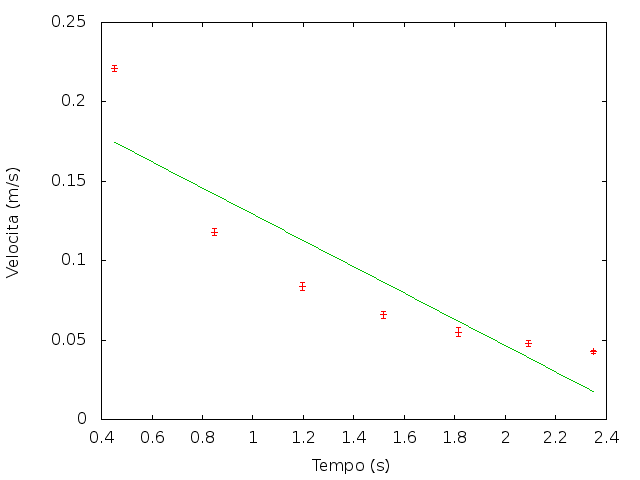
\includegraphics[width=0.8\textwidth]{velocita_30gradi_normale}
		\label{fig:30n}
	\end{figure}
	
	\subsection {Inclinazione 45', senza peso}
	\begin{figure}[H]
		\centering
		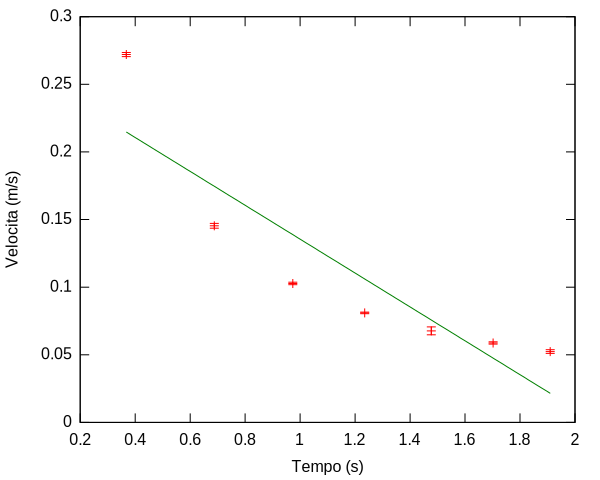
\includegraphics[width=0.8\textwidth]{velocita_45gradi_normale}
		\label{fig:45n}
	\end{figure}
 
	\subsection {Inclinazione 45', con peso}
		\begin{figure}[H]
		\centering
		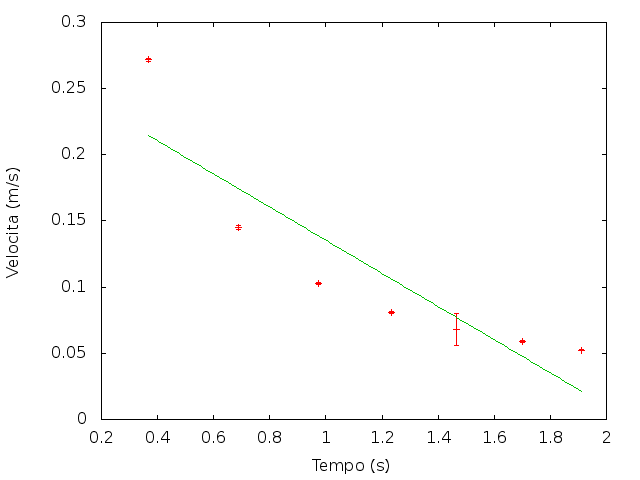
\includegraphics[width=0.8\textwidth]{velocita_45gradi_peso}
		\label{fig:45p}
	\end{figure}
 
	\subsection {Inclinazione 0', senza peso, senza spessore}
	\begin{figure}[H]
		\centering
		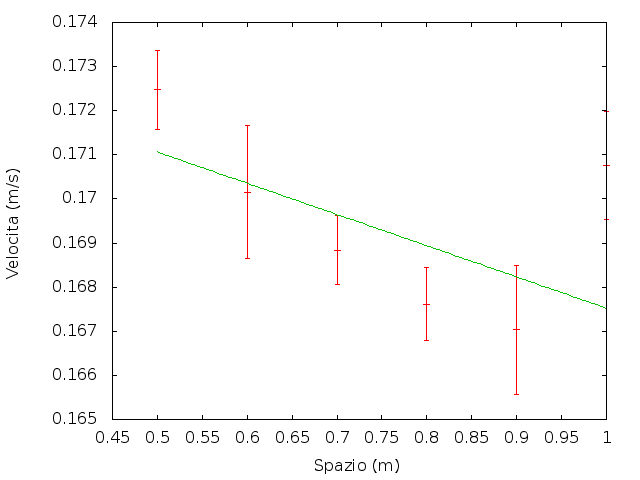
\includegraphics[width=0.8\textwidth]{velocita_0gradi_normale}
		\label{fig:0n}
	\end{figure}
	
	\subsection {Inclinazione 0', senza peso, con spessore}
	\begin{figure}[H]
		\centering
		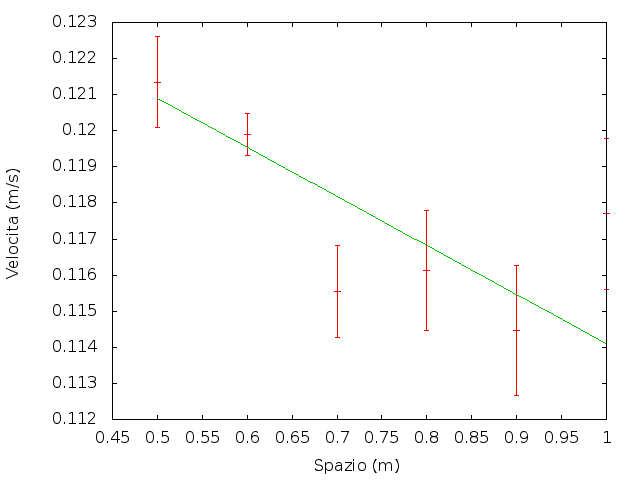
\includegraphics[width=0.8\textwidth]{velocita_0gradi_alluminio}
		\label{fig:0a}
	\end{figure}
 
 
	\subsection {Inclinazione 0', con peso, senza spessore}
		\begin{figure}[H]
		\centering
		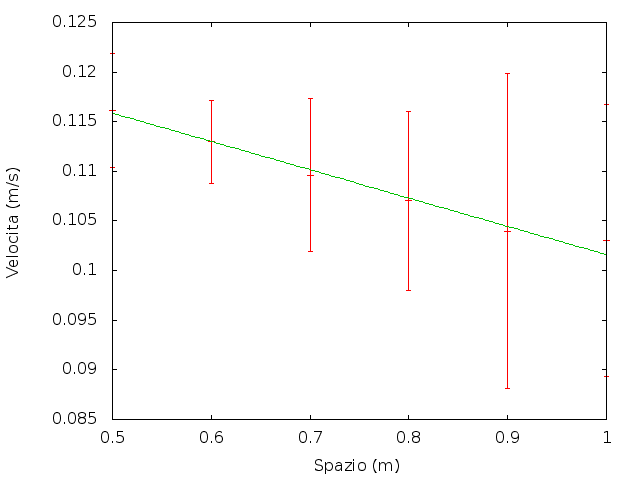
\includegraphics[width=0.8\textwidth]{velocita_0gradi_peso}
		\label{fig:0p}
	\end{figure}
 
	\subsection {Inclinazione 0', con peso, con spessore}
		\begin{figure}[H]
		\centering
		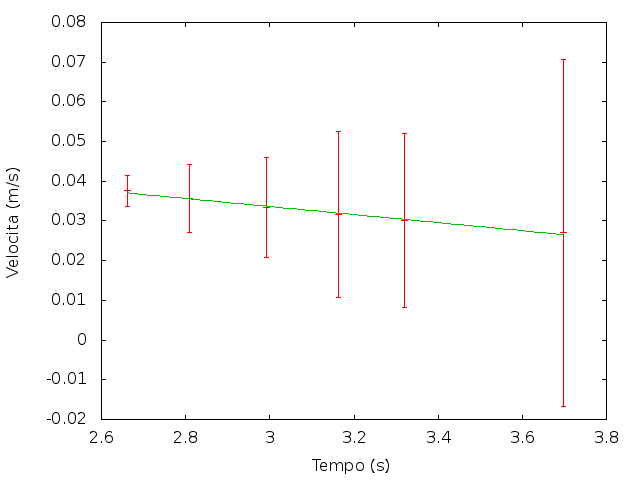
\includegraphics[width=0.8\textwidth]{velocita_0gradi_pesoalluminio}
		\label{fig:0ap}
	\end{figure}
 

\newpage
\section{Codice}

	Riportiamo in seguito il programma utilizzato per l'elaborazione dei dati. Fondalmentalmente abbiamo creato una
	classe template (una gerarchia, a dire la verità, ma non abbiamo usato le specializzazioni) che rappresenta
	una variabile statistica: contiene la media, la varianza del campione e quella della popolazione, la deviazione 
	standard del campione e quella della popolazione, il massimo, il minimo e l'errore della media. La classe base, 
	(la sola usata qui) legge i dati solo all'inizio nel costruttore, poi astrae da essi e grazie 
	all'overloading degli operatori di addizione, sottrazione, moltiplicazione e divisione, risulta facile ed efficiente 
	da manipolare: espressioni complesse di variabili statistiche, dato che i vari errori vengono propagati 
	dietro le quinte automaticamente, possono essere espresse chiaramente e concisamente nel codice, cosa che facilita il 
	controllo e velocizza la scrittura.
	%Verbatim non interpreta l'imput lasciando il testo com'è: ideale per inserire codice
	\begin{verbatim}
//============================================================================
// Name        : Misure.cpp
// Author      : Francesco Forcher
// Version     : 1.5
// Description : Programma per analizzare i dati sul pendolo raccolti in laboratorio
//============================================================================

/////////////////////////////////////////////////////////////////////////////////////
//Librerie
#include <iostream>//cin e cout
#include <fstream>//FileStream
#include <exception>//Eccezioni
#include <string>
#include <cstdlib>//system(clear)
#include <algorithm>//Sort?
#include <sstream>//StringStream

/////////////////////////////////////////////////////////////////////////////////////
//le mie classi

//In file "VarStat.h"
#pragma once//L'equivalente delle Include guards

#include <cmath>
#include <vector>
#include <algorithm>
#include <memory>
#include <limits>
#include <cmath>


#ifdef _MIO_DEBUG_

#include <iostream>//Per cerr

//Stampa il nome della variabile
#define VNAME(x) #x
#define VDUMP(x) std::clog << #x << " " << x << std::endl

#endif


//Il mio namespace
namespace mions {
//Classi per l'analisi dei dati statistici
namespace dataAnalisi {
using std::vector;

///////////////////////
//					 //
//	  VERSIONE 1.3	 //
//					 //
///////////////////////

///////////////////////////////////////////////////////////////////////////////////////////////////
/*
 * Forward declarations
 */
template <typename> class VarStat;//Forward declaration da usare nella funzione operator<<

template <typename T> const VarStat<T> operator*(const double& , const VarStat<T> );
template <typename T> const VarStat<T> operator*(const VarStat<T> , const double& );

///////////////////////////////////////////////////////////////////////////////////////////////////
//Versione
template <typename U>
std::ostream& operator <<(std::ostream& os, const VarStat<U>& rhs) {
	using namespace std;

	//Eclipse dà problemi con endl, modifichiamolo temporaneamente
	#define endl "\n"
	os << "Numero dati:                       " << rhs.getNumeroDatiEffettivo() << endl;
	os << "Media:                             " << rhs.getMedia() << endl;
	//cout << "Mediana:                           " << rhs.getMediana() << endl;
	os << "Varianza del campione:             " << rhs.getVarianzaCampione() << endl;
	os << "Deviazione standard campione:      " << rhs.getDeviazioneStandardCamp() << endl;
	os << "Varianza della popolazione:        " << rhs.getVarianzaPopolazione() << endl;
	os << "Deviazione standard popolazione:   " << rhs.getDeviazioneStandardPop() << endl;
	os << "Errore della media:                " << rhs.getErroreMedia() << endl;
	os << "Massimo:                           " << rhs.getMax() << endl;
	os << "Minimo:                            " << rhs.getMin() << endl;
	#undef endl

	return os;

}

//Moltiplicazione a destra per uno scalare
template <typename U>
inline const VarStat<U> operator*(const VarStat<U> lhs, const double& rhs) {
	VarStat<U> result = lhs; // Copia il primo oggettp
	result *= rhs;            // Aggiungici dentro l'altro
	return result;              // Ritorna il risultato
}

//Moltiplicazione a sinistra per uno scalare
template <typename U>
inline const VarStat<U> operator*(const double& lhs, const VarStat<U> rhs) {
	return (rhs*lhs);
}

//Moltiplicazione a sinistra per uno scalare

///////////////////////////////////////////////////////////////////////////////////////////////////
// Classe per l'analisi di UNA variabile statistica offline, cioè avendo accesso a tutti i dati fin dall'inizio
// O anche, che "rappresenta" una variabile statistica
template <class T>
class VarStat {
public:
	//vector<T> vectDati;
	//Funzioni overloaded
	friend std::ostream& operator<<<T>(std::ostream& , const VarStat<T>& );
	friend const VarStat<T> operator*<T>(const VarStat<T> , const double& );
	friend const VarStat<T> operator*<T>(const double& , const VarStat<T> );

	//
	VarStat(T valore) {
		iNumero_dati = 1;
		dMedia = (double)valore;
		dDeviazioneStandardCamp = 0;
		dDeviazioneStandardPop = 0;
		dVarianzaCampione = 0;
		dVarianzaPopolazione = 0;
		dMax = (double)valore;
		dMin = (double)valore;
		dErroreMedia = 0;
	}

	VarStat(T valore, double DevStdPop, int numDati = 100000) {
		iNumero_dati = numDati;
		dMedia = (double)valore;
		dDeviazioneStandardPop = DevStdPop;
		dDeviazioneStandardCamp = DevStdPop * sqrt(double(numDati-1)/double(numDati));
		dVarianzaCampione = dDeviazioneStandardCamp*dDeviazioneStandardCamp;
		dVarianzaPopolazione = DevStdPop*DevStdPop;
		dMax = (double)valore + DevStdPop;
		dMin = (double)valore - DevStdPop;
		dErroreMedia = DevStdPop / sqrt(numDati);
	}

	//Costruttore
	VarStat(const vector<T>& aDati, bool eliminaTreSigma = true) {
		//aDati = {1,2,3};//La classe ha una copia del vector! Non dei dati! Copiare un vector non è troppo impegnativo. O no? NOOO!!!
		int numDatiIniziale = aDati.size();
		vector<int> ListaDatifuori3Sigma; //0.003 = 100% - 99.7% = percentuale atttesa di fuori sigma, più spazio a caso

		//Se il vettore è vuoto la random variable è 0 +- 0 Buona idea?
		if (numDatiIniziale == 0) {

			#ifdef _MIO_DEBUG_
			std::clog << "Vettore vuoto, metto la variabile a zero+-zero";
			#endif

			iNumero_dati = 0;
			dMedia = 0;
			dDeviazioneStandardCamp = 0;
			dDeviazioneStandardPop = 0;
			dVarianzaCampione = 0;
			dVarianzaPopolazione = 0;
			dMax = 0;//Oppure +INFINITY
			dMin = 0;//O -INFINITY
			dErroreMedia = 0;
			return;
		}

		dMedia=(double)aDati[0];
		dMax=(double)aDati[0];
		dMin=(double)aDati[0];

		for(int i=0; i < numDatiIniziale; i++){
			//Media
			dMedia=(i*dMedia+(double)aDati[i])/(i+1);

			//Massimo e minimo (ottimizzabile?)
			dMax = (aDati[i] > dMax) ? aDati[i] : dMax;
			dMin = (aDati[i] < dMin) ? aDati[i] : dMin;
		}

		dVarianzaCampione=pow(((double)aDati[0]-dMedia),2);
		for(int i=0; i < numDatiIniziale; i++){
			//Varianza
			dVarianzaCampione=(i*dVarianzaCampione+pow(((double)aDati[i]-dMedia),2)) /
					(i+1);
		}

		dDeviazioneStandardCamp = sqrt(dVarianzaCampione);

		//se sigma2c=S/N e sigma2p=S/(N-1), allora, sostituendo S e risolvendo, sigma2p=sigma2c*N/(N-1)
		dVarianzaPopolazione = dVarianzaCampione*double(numDatiIniziale)/(double(numDatiIniziale)-1);
		iNumero_dati = aDati.size();
		////////////////////////////////////////////////////////////////////////////////////////////////////
		//Se eliminaTreSigma è true, rifai i conti togliendo i dati inaccettabili
		int numCancellazioni = 0;
		if (eliminaTreSigma){
			std::clog << "Elimino i dati oltre 3 sigma...\n" ;
			/* pDato è un tipo vector<double>::iterator, e si comporta come un puntatore a un elemento dell'array
			 * Sarebbe più leggibile scrivere "auto pDato = vectDati.begin();", ma per chiarezza mettiamo il tipo completo
			 *
			 * typename è richiesto perchè se qualcuno scrivesse "T::iterator * iter;" e se per esempio T contenesse un int chiamato iterator questa
			 * sarebbe una moltiplicazione (stupido c++), quindi dobbiamo specificare che intendiamo un tipo. Vedere:
			 * http://pages.cs.wisc.edu/~driscoll/typename.html#real_reason
			 *
			 * Non incrementiamo l'iteratore (pDato++) nell'istruzione for, invece lo assegnamo nel ciclo
			 */
			int i = 0;
			for (typename vector<T>::const_iterator pDato = aDati.begin();
					pDato != aDati.end();
					pDato++, i++)// i indica l'offset dall'inizio del vector, lo useremo dopo per verificare i dati
			{
				//i++;//Per mettere gli offset degli iterator, probabilmente si può mettere nel ciclo direttamente a questo punto
				if (abs(dMedia - (*pDato) ) >= 3*dDeviazioneStandardCamp) {
					/* Cancelliamo dal Vector i dati inaccettabili. Operazione costosa perchè i dati successivi vengono traslati
					 * indietro, ma è meglio un Vector di una LinkedList perchè i dati possono essere messi nella cache e occuma meno memoria.
					 * erase richiede un iterator, quindi siamo "costretti" a usarlo
					 */
					std::clog << "Eliminato dato: " << *pDato << "\n";

					ListaDatifuori3Sigma.push_back(i);//Aggiungi il dato nella posizione i alla lista degli "incriminati"

					numCancellazioni = numCancellazioni + 1;
				}
			}
			std::clog << "Cancellati " << numCancellazioni << " dati\n\n";
		}//EndIf
		////////////////////////////////////////////////////////////////////////////////////////////////////

		if ( !(ListaDatifuori3Sigma.empty())) {
			for (int k = 0; k < numCancellazioni; ++k) {
				std::cerr << ListaDatifuori3Sigma[k] << std::endl;
			}

			//Rifacciamo i conti
			numDatiIniziale = aDati.size();
			dMedia=(double)aDati[0];
			dMax=(double)aDati[0];
			dMin=(double)aDati[0];

			// j è l'indice del vettore che contiene gli indici dei dati da scartare. Ovviamente si suppone che questi siano ordinati e strettamente meno di numDatiIniziale
			int j = 0;
			for(int i=0; i < numDatiIniziale; i++) {
				//Media
				//Se il dato è buono prosegui coi calcoli
				if (i != *(ListaDatifuori3Sigma.begin() + j) ) {
					dMedia=(i*dMedia+(double)aDati[i])/(i+1);

					//Massimo e minimo
					dMax = (aDati[i] > dMax) ? aDati[i] : dMax;
					dMin = (aDati[i] < dMin) ? aDati[i] : dMin;
				} else {
					//Il dato è da scartare, prosegui con quello successivo (e avanza al prossimo numero nella lista, intanto)
					j++;
				}
			}

			// Di nuovo j
			j=0;
			dVarianzaCampione=pow(((double)aDati[0]-dMedia),2);
			for(int i=0; i < numDatiIniziale; i++) {
				//Varianza
				if (i != *(ListaDatifuori3Sigma.begin() + j)) {
					dVarianzaCampione=(i*dVarianzaCampione+pow(((double)aDati[i]-dMedia),2)) /
							(i+1);
				} else {
					j++;
				}
			}
			dDeviazioneStandardCamp = sqrt(dVarianzaCampione);

			//se sigma2c=S/N e sigma2p=S/(N-1), allora, sostituendo S e risolvendo, sigma2p=sigma2c*N/(N-1)
			dVarianzaPopolazione = dVarianzaCampione*double(numDatiIniziale)/(double(numDatiIniziale)-1);

		}//EndIf del ricalcolo
		////////////////////////////////////////////////////////////////////////////////////////////////////

		//Deviazione standard popolazione
		dDeviazioneStandardPop=sqrt(dVarianzaPopolazione);
		iNumero_dati = numDatiIniziale - ListaDatifuori3Sigma.size();
		dErroreMedia = dDeviazioneStandardPop / sqrt(iNumero_dati);

	}//Fine costruttore

	//Distruttore
	virtual ~VarStat() = default;//Virtual perchè devono ereditare da questa. Lecito il default? Bè compila

	//Getters
	inline double getMedia() const {return dMedia;};
	//Scarto Quadratico Medio (N)
	inline double getDeviazioneStandardCamp() const {return dDeviazioneStandardCamp;};
	//Errore Quadrato Medio N-1
	inline double getDeviazioneStandardPop() const {return dDeviazioneStandardPop;};
	//Su Excel sono invertite, cioè per varianza del campione io intendo la varianza propria dei dati
	inline double getVarianzaCampione() const {return dVarianzaCampione;}
	//Su Excel sono invertite, cioè per varianza popolazione io considero implicitamente i dati come un campione quindi
	//la varianzaPopolazione è calcolata fratto N-1
	inline double getVarianzaPopolazione() const {return dVarianzaPopolazione;}
	//double getMediana() ordina i dati come side effect
	//Tolta
	inline double getMax() const {return dMax;}
	inline double getMin() const {return dMin;}
	// Errore della media
	inline double getErroreMedia() const {return dErroreMedia;}
	long getNumeroDatiEffettivo() const {return iNumero_dati;}
	//Range della variabile
	inline long getRange() const {return dMax - dMin;}
	//double getModa() const {return dModa;}

	//Operatori
	//Somma una variabile statistica a un'altra e memorizzala nella prima. Vedi commento su -=, sotto
	inline VarStat<T>& operator+=(const VarStat<T>& rhs) {
		using std::abs;
		//Obiettivo: dare gli stessi risultati come se avessi sommato i dati di due insiemi (i dati due a due, non gli insiemi) ma senza un ordine definito tra i due
		//iNumero_dati = iNumero_dati; Non sto unendo gli insiemi di dati, ma sommando i singoli elementi fra loro
		dMedia += rhs.getMedia();//Somma le medie delle due variabili
		dVarianzaCampione = rhs.getVarianzaCampione() + getVarianzaCampione();//Propagazione dell'errore
		dVarianzaPopolazione = rhs.getVarianzaPopolazione() + getVarianzaPopolazione();

		//La nuova varianza permette di calcolare direttamente la nuova std
		dDeviazioneStandardCamp = sqrt(getVarianzaCampione());
		dDeviazioneStandardPop = sqrt(getVarianzaPopolazione());

		// Il massimo della somma è la somma dei due massimi
		// Worst-case max? Non ben definito, ma se ho due set di dati, il massimo (tra tutte le possibilità) è la somma dei due massimi precedenti
		dMax = rhs.getMax() + getMax();

		//Idem per il minimo, il minimo "minore" è la somma dei minimi
		dMin = rhs.getMin() + getMin();

		dErroreMedia = sqrt(pow(rhs.getErroreMedia(),2) + pow(getErroreMedia(),2));
		return *this;	//Idiozia ma dicono che serva
	}

	//Sottrai una variabile statistica a un'altra e memorizzala nella prima. v1 -= v2 è come v.operator-=(v2), quindi le funzioni get, etc qui dentro si riferiscono a v1!!! E rhs.get... a v2

	inline VarStat<T>& operator-=(const VarStat<T>& rhs) {
		using std::abs;
		//TODO: Possibile farlo come lhs += (-1)*rhs ?
		//Obiettivo: dare gli stessi risultati come se avessi sottratto i dati di due insiemi (i dati due a due, non gli insiemi) ma senza un ordine definito tra i due
		//iNumero_dati = iNumero_dati; Non sto unendo gli insiemi di dati, ma sottraendo i singoli elementi fra loro
		dMedia = getMedia() - rhs.getMedia();//Sottrai le medie delle due variabili
		dVarianzaCampione = getVarianzaCampione() + rhs.getVarianzaCampione();//Propagazione dell'errore
		dVarianzaPopolazione = getVarianzaPopolazione() + rhs.getVarianzaPopolazione();

		//La nuova varianza permette di calcolare direttamente la nuova std
		dDeviazioneStandardCamp = sqrt(getVarianzaCampione());
		dDeviazioneStandardPop = sqrt(getVarianzaPopolazione());

		//Worst-case min
		// Il massimo della differenza è la differenza tra il valore più alto del minuendo e quello più basso del sottraendo
		dMax = getMax() - rhs.getMin();

		//Il minimo "minore" è il minimo del minuendo a cui abbiamo tolto il più possibile, cioè il massimo del sottraendo
		dMin = getMin() - rhs.getMax();

		dErroreMedia = sqrt(pow(rhs.getErroreMedia(),2) + pow(getErroreMedia(),2));
		return *this;	//Idiozia ma dicono che serva
	}


	//%%%%%%%%%%%%%%%%%%%%%%%%%%%%%%%%%%%%%%%%%%%%%%%%%%%%%%%%%%%%%%%%%%%%%%%%%%%%%%%%%%%%%%%%%%%%%%%%%%%%%%%
	//%%%%%%%%%%%%%%%%%%%%%%%%%%%%%%%%%%%%%%%%%%%%%%%%%%%%%%%%%%%%%%%%%%%%%%%%%%%%%%%%%%%%%%%%%%%%%%%%%%%%%%%
	//Operatori
	//moltiplica una variabile statistica a un'altra e memorizzala nella prima. Vedi commento su -=, sotto
	inline VarStat<T>& operator*=(const VarStat<T>& rhs) {
		using std::abs;
		//Obiettivo: dare gli stessi risultati come se avessi moltiplicato i dati di due insiemi (i dati due a due, non gli insiemi) ma senza un ordine definito tra i due
		//iNumero_dati = iNumero_dati; Non sto unendo gli insiemi di dati, ma moltiplicando i singoli elementi fra loro
		double tMedia = getMedia();//Salvo la media
		dMedia = rhs.getMedia() * getMedia();//MOltiplica le medie delle due variabili
		dVarianzaCampione = getMedia()*getMedia()*(getVarianzaCampione() / (tMedia*tMedia) + rhs.getVarianzaCampione() / (rhs.getMedia() * rhs.getMedia()) );//Propagazione dell'errore
		dVarianzaPopolazione = getMedia()*getMedia()*(getVarianzaPopolazione() / (tMedia*tMedia) + rhs.getVarianzaPopolazione() / (rhs.getMedia() * rhs.getMedia()) );

		//La nuova varianza permette di calcolare direttamente la nuova std
		dDeviazioneStandardCamp = sqrt(getVarianzaCampione());
		dDeviazioneStandardPop = sqrt(getVarianzaPopolazione());

		// Il massimo della somma è la somma dei due massimi
		// Worst-case max? Non ben definito, ma se ho due set di dati, il massimo (tra tutte le possibilità) è la somma dei due massimi precedenti
		// TODO: Casi non maggiori di zero
		// TODO: Casi non maggiori di zero
		dMax = (getMedia() > 0) ? (getMax() * rhs.getMax()) : ( INFINITY );

		//Idem per il minimo, il minimo "minore" è la somma dei minimi
		dMin = (getMedia() > 0) ? (getMin() * rhs.getMin()) : ( -INFINITY );

		dErroreMedia = getDeviazioneStandardPop() / sqrt(getNumeroDatiEffettivo());//Propagato come una StDev normale
		return *this;	//Idiozia ma dicono che serva
	}

	inline VarStat<T>& operator/=(const VarStat<T>& rhs) {
		using std::abs;
		//Obiettivo: dare gli stessi risultati come se avessi moltiplicato i dati di due insiemi (i dati due a due, non gli insiemi) ma senza un ordine definito tra i due
		//iNumero_dati = iNumero_dati; Non sto unendo gli insiemi di dati, ma moltiplicando i singoli elementi fra loro
		double tMedia = getMedia();//Salvo la media
		dMedia = getMedia() / rhs.getMedia();//MOltiplica le medie delle due variabili
		dVarianzaCampione = getMedia() * getMedia()*(getVarianzaCampione() / (tMedia*tMedia) + rhs.getVarianzaCampione() / (rhs.getMedia() * rhs.getMedia()) );//Propagazione dell'errore
		dVarianzaPopolazione = getMedia() * getMedia()*(getVarianzaPopolazione() / (tMedia*tMedia) +rhs.getVarianzaPopolazione() / (rhs.getMedia() * rhs.getMedia()) );

		//La nuova varianza permette di calcolare direttamente la nuova std
		dDeviazioneStandardCamp = sqrt(getVarianzaCampione());
		dDeviazioneStandardPop = sqrt(getVarianzaPopolazione());

		// Il massimo della somma è la somma dei due massimi
		// Worst-case max? Non ben definito, ma se ho due set di dati, il massimo (tra tutte le possibilità) è la somma dei due massimi precedenti
		// TODO: Casi non maggiori di zero
		dMax = (getMedia() > 0) ? (getMax() / rhs.getMin()) : ( INFINITY );

		//Idem per il minimo, il minimo "minore" è la somma dei minimi
		dMin = (getMedia() > 0) ? (getMin() / rhs.getMax()) : ( -INFINITY );

		dErroreMedia = getDeviazioneStandardPop() / sqrt(getNumeroDatiEffettivo());
		return *this;	//Idiozia ma dicono che serva
	}








	//Moltiplicazione per scalare, compound assignment. v *= d è come v.operator*=(d), quindi le funzioni get, etc qui dentro si riferiscono a v
	inline VarStat<T>& operator*=(const double& rhs) {
		using std::abs;
		//Obiettivo: dare gli stessi risultati come se avessi preso tutti i dati e, moltiplicato ciascuno per rhs, li avessi passati a lhs
		dMedia = rhs * getMedia();//Moltiplica la media della VarStat a sinistra del simbolo per il double a destra
		dVarianzaCampione = rhs * rhs * getVarianzaCampione();
		dVarianzaPopolazione = rhs * rhs * getVarianzaPopolazione();
		dDeviazioneStandardCamp = abs(rhs) * getDeviazioneStandardCamp();
		dDeviazioneStandardPop = abs(rhs) * getDeviazioneStandardPop();

		//Se moltiplico per uno scalare negativo, il minimo nei positivi diventa il massimo nei negativi (es se min=-20 e max=40, se li moltiplico per -2 allora min=-40 e max=20)
		T tMax = dMax;//Massimo temporaneo, perchè quando calcoliamo dMin è già stato modificato dmax
		T tMin = dMin;
		dMax = (rhs >= 0 ? rhs * tMax : rhs * tMin);
		dMin = (rhs >= 0 ? rhs * tMin : rhs * tMax);

		dErroreMedia = abs(rhs)*getErroreMedia();
		return *this;	//Idiozia ma dicono che serva
	}

	//Somma di due VarStat
	//Trucchetto per riutilizzare il lavoro svolto con +=
	const VarStat<T> operator+(const VarStat<T> &other) const {
		VarStat<T> result = *this; // Copia il primo oggettp
		result += other;            // Aggiungici dentro l'altro
		return result;              // Ritorna il risultato
	}

	//Sottrazione di due VarStat
	//Trucchetto per riutilizzare il lavoro svolto con -=
	const VarStat<T> operator-(const VarStat<T>& other) const {
		VarStat<T> result = *this; // Copia il primo oggettp
		result -= other;            // Aggiungici dentro l'altro
		return result;              // Ritorna il risultato
	}

	const VarStat<T> operator*(const VarStat<T>& other) const {
		VarStat<T> result = *this; // Copia il primo oggettp
		result *= other;            // Aggiungici dentro l'altro
		return result;              // Ritorna il risultato
	}

	const VarStat<T> operator/(const VarStat<T>& other) const {
		VarStat<T> result = *this; // Copia il primo oggettp
		result /= other;            // Aggiungici dentro l'altro
		return result;              // Ritorna il risultato
	}


	//Moltiplicazione per uno scalare
	//Trucchetto per riutilizzare il lavoro svolto con *= double,
//	const VarStat<T> operator*(const double rhs) const {
//		VarStat<T> result = *this; // Copia il primo oggettp
//		result *= rhs;            // Aggiungici dentro l'altro
//		return result;              // Ritorna il risultato
//	}

private:

	double dMedia = -INFINITY;
	double dDeviazioneStandardCamp = -INFINITY;
	double dDeviazioneStandardPop = -INFINITY;
	double dVarianzaCampione = -INFINITY;
	double dVarianzaPopolazione = -INFINITY;
	//double dMediana = -INFINITY;
	double dMax = -INFINITY;
	double dMin = -INFINITY;
	double dErroreMedia = -INFINITY;
	int iNumero_dati = 0;
	//double dModa=0;

};




}//Fine DataAnalisi

}//Fine del mio namespace


//In file "SortingVarStat.h"
/*
 * SortingVarStat.h
 *
 *  Created on: Feb 19, 2014
 *      Author: francesco
 */

#ifndef SORTINGVARSTAT_H_
#define SORTINGVARSTAT_H_

#include "VarStat.h"

///////////////////////
//					 //
//	  VERSIONE 0.1	 //
//					 //
///////////////////////


namespace mions {
namespace dataAnalisi {

template <typename> class Sorting_VarStat;

//Notare come non sia const Sorting_VarStat<U>&, poichè la mediana non viene calcolata finchè non serve, quindi getMediana() potrebbe modificare l'oggetto
template <typename U>
std::ostream& operator <<(std::ostream& os, Sorting_VarStat<U>& rhs) {
	using namespace std;

	//Eclipse dà problemi con endl, modifichiamolo temporaneamente
	#define endl "\n"
	os << "Numero dati:                       " << rhs.getNumeroDatiEffettivo() << endl;
	os << "Media:                             " << rhs.getMedia() << endl;
	os << "Mediana:                           " << rhs.getMediana() << endl;
	os << "Varianza del campione:             " << rhs.getVarianzaCampione() << endl;
	os << "Deviazione standard campione:      " << rhs.getDeviazioneStandardCamp() << endl;
	os << "Varianza della popolazione:        " << rhs.getVarianzaPopolazione() << endl;
	os << "Deviazione standard popolazione:   " << rhs.getDeviazioneStandardPop() << endl;
	os << "Errore della media:                " << rhs.getErroreMedia() << endl;
	os << "Massimo:                           " << rhs.getMax() << endl;
	os << "Minimo:                            " << rhs.getMin() << endl;
	#undef endl

	return os;
	};

template <class T>
class Sorting_VarStat: public mions::dataAnalisi::VarStat<T> {
public:
	friend std::ostream& operator<<<T>(std::ostream& os, Sorting_VarStat<T>& rhs);

	vector<T> vectDati;
	Sorting_VarStat(const vector<T>&& aDati, bool eliminaTreSigma = true) : mions::dataAnalisi::VarStat<T>(aDati, eliminaTreSigma) {
		vectDati = aDati;//Copiati i dati, così puoi riordinarli in santa pace. In teoria move-assignment
	};

	virtual ~Sorting_VarStat() throw() {};

	double getMediana() {
		if (dMediana != -INFINITY) {
			return dMediana;
		}
		else
		{
			ordinaDati();
			int numDati = this->getNumeroDatiEffettivo();
			if (numDati % 2 == 1) {
				return dMediana = (double)vectDati[(numDati-1)/2];
			} else {
				return dMediana = (double)(vectDati[numDati/2-1]+vectDati[numDati/2])/2;
			}
		}
	}

///////////////////////////////////////////////////////////////////////////////////////////////
private:

	bool DatiOrdinati = false;
	double dMediana = -INFINITY;//Un valore che non dovrebbe assumere mai...


	inline void ordinaDati() {
		if (!DatiOrdinati) {
			std::sort(vectDati.begin(),vectDati.end());
			DatiOrdinati = true;
		}
	}
};

} /* namespace dataAnalisi */
} /* namespace mions */

#endif /* SORTINGVARSTAT_H_ */



#define VERSIONE 1.5

/////////////////////////////////////////////////////////////////////////////////////
//Prototipi

/////////////////////////////////////////////////////////////////////////////////////
//Il primo argomento è la cartella dei dati
int main(int numParam, char* args[]) {

	using namespace std;

	system("clear");
	cout << "\n";
	cout << "Programma per analizzare i dati della guidovia, versione: " << VERSIONE << endl;
	//Ricordarsi che con 0 gradi l'intervallo era di 20!
	const int NUM_FILE = 7;// 7 file (7 intervalli) per 15, 30, 45 gradi
	const int NUM_FILE_0GRADI = 6; //  file per 60,70,80,90,100,110
	const int NUM_DATIPERFILE = 5;// 5 dati in ogni file
	const int ANGOLI_NUM = 3;//15, 30, 45 0 e 45 li facciamo a parte
	//const auto INTERVALLO = VarStat<double>(0.1, 0.001 / sqrt(6));//Distribuzione triangolare

	try {
		//stringstream ss;
		string nf;//Nome file da aprire
		//FileStream
		ofstream FileMedie;//FileStream
		ofstream FileRiassunto;
		using namespace mions::dataAnalisi;
		vector<VarStat<double> > arrayRiassunti;//Contiene le informazioni come la deviazione standard, etc
		vector<VarStat<double> > arrayTempi;
		arrayRiassunti.reserve(NUM_FILE);
		const auto INTERVALLO_PV = VarStat<double>(0.1, 0.001 / sqrt(6));//Distribuzione triangolare

//		vector<double> v1 = {1,1,1,100000,1,1,1,1,1,1,1,1,1,1,1,1,1,1,1,1,1,1,1,1,1,1,1,1,1,1,2,3,4,2,1,3,2};
//
//		vector<double> v2 = {3,4,7,8};
//		vector<double> v3 = {1,2,5,6};
//		VarStat<double> var2(v2,true);
//		VarStat<double> var3(v3,true);
//
//		VarStat<double> AnDat(v2,true);
//		//Sorting_VarStat<double> var2(std::move(v3));//Non usare più v1
//		//cout << "MEDIANA " <<var2.getMediana() << "\n";
//		AnDat = (AnDat-var2)/(AnDat*3*var2);
//		cout << "var2: \n" << var2 << endl;
//		cout << "var3: \n" << var3 << endl;
//		cout << "somma elementi: \n" << VarStat<double>({4,6,12,14}) << endl;
//		cout << "somma variabili: \n" << (var2+var3) << endl;
//
//		return 0;


//Prima esperianza, guidovia inclinata a 15, 30 e 45 gradi senza peso
///////////////////////////////////////////////////////////////////////////////////////////////////
		{

		//stringstream ss;
		string nf;//Nome file da aprire
		//FileStream
		ofstream FileMedie;//FileStream
		ofstream FileRiassunto;
		ofstream FileVelocita;
		using namespace mions::dataAnalisi;
		vector<VarStat<double> > arrayRiassunti;//Contiene le informazioni come la deviazione standard, etc
		vector<VarStat<double> > arrayTempi;

		arrayRiassunti.reserve(NUM_FILE);
		string nomeoutputfile;
		string nomefilemedie;
		string nomefilevelocita;
		string nomeoutputvelocita;//Per tenere temporaneamente la variabile ed evitare il self assignment

		/* Vari casi:
		 * 	1. nè peso nè alluminio
		 */
		string tipodati;
				nomeoutputfile = "./Risultati/normale_dati.txt";
				//tipodati = "d";
				nomefilemedie = "arrayTempi_PrimaVolta_normale.txt";
				nomefilevelocita = "velocita_PV_normale.txt";//PV = prima volta

		FileRiassunto.open(nomeoutputfile.c_str());

		for (int angoli = 1; angoli <= ANGOLI_NUM; angoli++) {
			//TODO aggiunto zero all'inizio
			arrayTempi.emplace_back(0.0);

			for (int intervallo = 1; intervallo <= NUM_FILE; intervallo++) {

				stringstream ss;
				ifstream FileImputDati;//File di imput
				ss << "./DatiFormattati/DatiStandardizzati/";
				ss << "d";//Tipo dei dati contenuti nel file: d, cd
				ss << intervallo*10 + 40;
				ss << "_";
				ss << angoli*15;
				ss >> nf;
				//ss.flush();


				clog << nf << endl;
				FileImputDati.open(nf.c_str());//Apro il file indicato nell'argomento dato via shell
				if (!FileImputDati.is_open())
					throw "Errore: file non aperto";

				vector<double> tempVect(5);// Vector che contiene i dati di un file solo, da cui ricavare il tempo medio
				tempVect.reserve(NUM_DATIPERFILE);

				clog << tempVect.size() << endl;
				for (unsigned int i = 0; i < tempVect.size(); i++) {
					FileImputDati >> tempVect[i];
					clog << "Pos " << i << ": " << tempVect[i] << endl;
				}
				clog << "Dati letti. Analizzo..." << endl << endl;

				arrayRiassunti.emplace_back(tempVect,true);// Forwarda gli argomenti a un oggetto costruito DIRETTAMENTE nel vettore (cioè, manda gli argomenti VarStat dentro al vettore)

				cout << endl;
				cout << "Nome file: " << nf << endl;
				cout << arrayRiassunti.back();

				FileRiassunto << endl;
				FileRiassunto << "Nome file: " << nf << endl;
				FileRiassunto << arrayRiassunti.back() << endl;

				arrayTempi.emplace_back(arrayRiassunti.back());

				ss.clear();
				FileImputDati.close();
			}//Intervalli


			switch (angoli) {
				case 1:
					//Ricicliamo nomeoutputfile per indicare i file di uscita
					nomeoutputfile = string("./Risultati/MetaDati/15/") + nomefilemedie;
					nomeoutputvelocita = string("./Risultati/MetaDati/15/") + nomefilevelocita;
					FileMedie.open(nomeoutputfile.c_str());
					FileVelocita.open(nomeoutputvelocita.c_str());
					//const auto intervallo = VarStat<double>(0.1, 0.1 / sqrt(6));
					for (int i = 0; i < NUM_FILE; i++)
					{
						FileMedie << ((arrayTempi[i+1]+arrayTempi[i])/2).getMedia() << endl;//sette medie di cinque tempi ciascuns
						FileVelocita << (INTERVALLO_PV / (arrayTempi[i+1] - arrayTempi[i]) ).getMedia() << " "
								<< (INTERVALLO_PV / (arrayTempi[i+1] - arrayTempi[i]) ).getDeviazioneStandardPop() << endl;//10 cm di intervallo/cinque_tempi_media << endl;//10 cm di intervallo
					}
					FileMedie.close();
					FileVelocita.close();
					break;
				case 2:
					//Ricicliamo nomeoutputfile per indicare i file di uscita
					nomeoutputfile = string("./Risultati/MetaDati/30/") + nomefilemedie;
					nomeoutputvelocita = string("./Risultati/MetaDati/30/") + nomefilevelocita;
					FileMedie.open(nomeoutputfile.c_str());
					FileVelocita.open(nomeoutputvelocita.c_str());
					for (int i = 0; i < NUM_FILE; i++)
					{
						FileMedie << ( (arrayTempi[i+1] + arrayTempi[i]) / 2 ).getMedia() << endl;//sette medie di cinque tempi ciascuns
						FileVelocita << (INTERVALLO_PV / (arrayTempi[i+1] - arrayTempi[i]) ).getMedia() << " "
								<< (INTERVALLO_PV / (arrayTempi[i+1] - arrayTempi[i]) ).getDeviazioneStandardPop() << endl;//10 cm di intervallo/cinque_tempi_media << endl;//10 cm di intervallo
					}
					FileMedie.close();
					FileVelocita.close();
					break;
				case 3:
					//Ricicliamo nomeoutputfile per indicare i file di uscita
					nomeoutputfile = string("./Risultati/MetaDati/45/") + nomefilemedie;
					nomeoutputvelocita = string("./Risultati/MetaDati/45/") + nomefilevelocita;
					FileMedie.open(nomeoutputfile.c_str());
					FileVelocita.open(nomeoutputvelocita.c_str());
					for (int i = 0; i < NUM_FILE; i++)
					{
						FileMedie << ((arrayTempi[i+1]+arrayTempi[i])/2).getMedia() << endl;//sette medie di cinque tempi ciascuns
						FileVelocita << (INTERVALLO_PV / (arrayTempi[i+1] - arrayTempi[i]) ).getMedia() << " "
								<< (INTERVALLO_PV / (arrayTempi[i+1] - arrayTempi[i]) ).getDeviazioneStandardPop() << endl;//10 cm di intervallo/cinque_tempi_media << endl;//10 cm di intervallo
					}
					FileMedie.close();
					FileVelocita.close();
					break;
				default:
					throw "Errore: numero casi angoli sbagliato";
					break;
			}//switch
			arrayTempi.clear();
		}//Angoli

		FileRiassunto.close();
		arrayRiassunti.clear();
	  }//Blocco prima esperienza senza peso
///////////////////////////////////////////////////////////////////////////////////////////////////










//Prima esperianza, guidovia inclinata a 45 con peso
///////////////////////////////////////////////////////////////////////////////////////////////////
		/*
		 * Vari casi:
		 * 	1. nè peso nè alluminio
		 * 	2. peso
		 */
//for (int varicasi = 1; varicasi <= 2; varicasi++)
		{

			string nf;						// Nome file
			ofstream FileMedie;				// File con le medie dei tempi
			ofstream FileRiassunto;			// File con le informazioni sulle cinquine di dati
			ofstream FileVelocita;
			using namespace mions::dataAnalisi;
			vector<VarStat<double> > arrayRiassunti;//Contiene le informazioni come la deviazione standard, etc
			vector<VarStat<double> > arrayTempi;
			//TODO aggiunto zero all'inizio
			arrayTempi.emplace_back(0.0);

			arrayRiassunti.reserve(NUM_FILE);
			string nomeoutputfile;
			string nomefilemedie;
			string nomefilevelocita;
			string nomeoutputvelocita;


				string tipodati;
				nomeoutputfile = "./Risultati/peso_dati.txt";
				tipodati = "cd";
				nomefilemedie = "arrayTempi_PrimaVolta_peso.txt";
				nomefilevelocita = "velocita_PV_peso.txt";


			//string nomeoutputfile = "./Risultati/nopeso_dati.txt";
			FileRiassunto.open(nomeoutputfile.c_str());
				for (int intervallo = 1; intervallo <= NUM_FILE; intervallo++) {

					stringstream ss;
					ifstream FileImputDati;					//File di imput
					ss << "./DatiFormattati/DatiStandardizzati/";
					ss << tipodati;	//Tipo dei dati contenuti nel file: d, cd
					ss << intervallo * 10 + 40;
					ss << "_";
					ss << "45";
					ss >> nf;
					//ss.flush();

					clog << nf << endl;
					FileImputDati.open(nf.c_str());	//Apro il file indicato nell'argomento dato via shell
					if (!FileImputDati.is_open())
						throw "Errore: file non aperto";

					vector<double> tempVect(5);	// Vector che contiene i dati di un file solo, da cui ricavare il tempo medio
					tempVect.reserve(NUM_DATIPERFILE);

					clog << tempVect.size() << endl;
					for (unsigned int i = 0; i < tempVect.size(); i++) {
						FileImputDati >> tempVect[i];
						clog << "Pos " << i << ": " << tempVect[i] << endl;
					}
					clog << "Dati letti. Analizzo..." << endl << endl;

					arrayRiassunti.emplace_back(tempVect, true);// Forwarda gli argomenti a un oggetto costruito DIRETTAMENTE nel vettore (cioè, manda gli argomenti VarStat dentro al vettore)

					cout << endl;
					cout << "Nome file: " << nf << endl;
					cout << arrayRiassunti.back();

					FileRiassunto << endl;
					FileRiassunto << "Nome file: " << nf << endl;
					FileRiassunto << arrayRiassunti.back() << endl;

					arrayTempi.emplace_back(arrayRiassunti.back());

					ss.clear();
					FileImputDati.close();
				}//Intervalli

				//Ex switch
					//Ricicliamo nomeoutputfile per indicare i file di uscita
					nomeoutputfile = string("./Risultati/MetaDati/45/")
							+ nomefilemedie;
					nomeoutputvelocita = string("./Risultati/MetaDati/45/")
							+ nomefilevelocita;
					FileMedie.open(nomeoutputfile.c_str());
					FileVelocita.open(nomeoutputvelocita.c_str());
					for (int i = 0; i < NUM_FILE; i++)
					{
						FileMedie << ((arrayTempi[i+1]+arrayTempi[i])/2).getMedia() << endl;//sette medie di cinque tempi ciascuns
						FileVelocita << (INTERVALLO_PV / (arrayTempi[i+1] - arrayTempi[i]) ).getMedia() << " "
								<< (INTERVALLO_PV / (arrayTempi[i+1] - arrayTempi[i]) ).getDeviazioneStandardPop() << endl;//10 cm di intervallo/cinque_tempi_media << endl;//10 cm di intervallo
					}
					FileMedie.close();
					FileVelocita.close();

			arrayTempi.clear();

			FileRiassunto.close();
			arrayRiassunti.clear();
		}					//Blocco prima esperienza 45 con peso
///////////////////////////////////////////////////////////////////////////////////////////////////
///////////////////////////////////////////////////////////////////////////////////////////////////
///////////////////////////////////////////////////////////////////////////////////////////////////















//%%%%%%%%%%%%%%%%%%%%%%%%%%%%%
// Seconda giornata %
//%%%%%%%%%%%%%%%%%%%%%%%%%%%%%

///////////////////////////////////////////////////////////////////////////////////////////////////
///////////////////////////////////////////////////////////////////////////////////////////////////
///////////////////////////////////////////////////////////////////////////////////////////////////
//Seconda esperienza, 0 gradi con alluminio e peso
		/* Vari casi:
		 * 	1. nè peso nè alluminio (file "d...")
		 * 	2. peso (file "cd...")
		 * 	4. alluminio
		 * 	3. peso e alluminio ("cad...")
		 */
		for (int varicasi = 1; varicasi <= 4; varicasi++)
		{
			string nf;						//Nome file da aprire
			ofstream FileMedie;				//File per le medie
			ofstream FileRiassunto;
			ofstream FileVelocita;
			using namespace mions::dataAnalisi;
			vector<VarStat<double> > arrayRiassunti;//Contiene le informazioni come la deviazione standard, etc
			vector<VarStat<double> > arrayTempi;//Niente zero perchè non devo dividere per la differenza
			arrayRiassunti.reserve(NUM_FILE_0GRADI);
			string nomeoutputfile;
			string nomefilemedie;
			string nomefilevelocita;
			string nomeoutputvelocita;
			const auto INTERVALLO_SV = VarStat<double>(0.2, 0.001 / sqrt(6));//Distribuzione triangolare


			/* Vari casi:
			 * 	1. nè peso nè alluminio (file "d...")
			 * 	2. peso (file "cd...")
			 * 	4. alluminio
			 * 	3. peso e alluminio ("cad...")
			 */
			string tipodati;
			switch (varicasi) {
				case 1: // normale
					nomeoutputfile = "./Risultati/normale_0gradi_dati.txt";
					tipodati = "d";
					nomefilemedie = "arrayTempi_0gradi_normale.txt";
					nomefilevelocita = "velocita_0gradi_normale.txt";
					break;
				case 2: // peso
					nomeoutputfile = "./Risultati/peso_0gradi_dati.txt";
					tipodati = "cd";
					nomefilemedie = "arrayTempi_0gradi_peso.txt";
					nomefilevelocita = "velocita_0gradi_peso.txt";
					break;
				case 3: // alluminio
					nomeoutputfile = "./Risultati/alluminio_0gradi_dati.txt";
					tipodati = "ad";
					nomefilemedie = "arrayTempi_0gradi_alluminio.txt";
					nomefilevelocita = "velocita_0gradi_alluminio.txt";
					break;
				case 4: // normale
					nomeoutputfile = "./Risultati/pesoalluminio_0gradi_dati.txt";
					tipodati = "cad";
					nomefilemedie = "arrayTempi_0gradi_pesoalluminio.txt";
					nomefilevelocita = "velocita_0gradi_pesoalluminio.txt";
					break;
				default:
					throw "Errore: Seconda esperienza: variante non nota";
					break;
			}

			FileRiassunto.open(nomeoutputfile.c_str());

			for (int intervallo = 1; intervallo <=  NUM_FILE_0GRADI; intervallo++) {
				stringstream ss;
				ifstream FileImputDati;					//File di input
				ss << "./DatiFormattati/DatiStandardizzati/";
				ss << tipodati;	//Tipo dei dati contenuti nel file: d, cd, ad, cad
				ss << intervallo * 10 + 50;
				ss << "_";
				ss << "0";
				ss >> nf;
				//ss.flush();

				clog << nf << endl;
				FileImputDati.open(nf.c_str());	//Apro il file indicato nell'argomento dato via shell
				if (!FileImputDati.is_open())
					throw "Errore: file non aperto";

				vector<double> tempVect(5);	// Vector che contiene i dati di un file solo, da cui ricavare il tempo medio
				tempVect.reserve(NUM_DATIPERFILE);

				clog << tempVect.size() << endl;
				for (unsigned int i = 0; i < tempVect.size(); i++) {
					FileImputDati >> tempVect[i];
					clog << "Pos " << i << ": " << tempVect[i] << endl;
				}
				clog << "Dati letti. Analizzo..." << endl << endl;

				arrayRiassunti.emplace_back(tempVect, true);// Forwarda gli argomenti a un oggetto costruito DIRETTAMENTE nel vettore (cioè, manda gli argomenti VarStat dentro al vettore)

				cout << endl;
				cout << "Nome file: " << nf << endl;
				cout << arrayRiassunti.back();

				FileRiassunto << endl;
				FileRiassunto << "Nome file: " << nf << endl;
				FileRiassunto << arrayRiassunti.back() << endl;

				arrayTempi.emplace_back(arrayRiassunti.back());

				ss.clear();
				FileImputDati.close();
			}					//Intervalli

			//Ex switch
				//Ricicliamo nomeoutputfile per indicare i file di uscita
				nomeoutputfile = string("./Risultati/MetaDati/0/")
						+ nomefilemedie;//Nomefilemedie scelto all'inizio nello switch
				nomeoutputvelocita = string("./Risultati/MetaDati/0/")
						+ nomefilevelocita;//Idem per nomefilevelocita
				FileMedie.open(nomeoutputfile.c_str());
				FileVelocita.open(nomeoutputvelocita.c_str());
				for (int i = 0; i < NUM_FILE_0GRADI; i++)
				{
					//Qui non c'è lo zero, quindi niente media
					FileMedie << (arrayTempi[i]).getMedia() << endl;//sette medie di cinque tempi ciascuns
					FileVelocita << (INTERVALLO_SV / arrayTempi[i]).getMedia() << " "
							<< (INTERVALLO_SV / arrayTempi[i]).getDeviazioneStandardPop() << endl;//10 cm di intervallo/cinque_tempi_media << endl;//10 cm di intervallo
				}
				FileMedie.close();
				FileVelocita.close();

		arrayTempi.clear();
		FileRiassunto.close();
		arrayRiassunti.clear();

		}
///////////////////////////////////////////////////////////////////////////////////////////////////
///////////////////////////////////////////////////////////////////////////////////////////////////
///////////////////////////////////////////////////////////////////////////////////////////////////










//////////////////////////////////////////////////
//Analizza i dati per la gravità
typedef VarStat<double> vs;
const double G15 = 0.25*M_PI/180.0;//15 primi di grado
const double G30 = 0.50*M_PI/180.0;//15 primi di grado
const double G45 = 0.75*M_PI/180.0;//15 primi di grado

ofstream AnalisiGravita;
AnalisiGravita.open("./Risultati/Analisi_Dati/DatiGravità");

////Media tra gravità a 15, 30, 45, 45peso presi dai valori di Gnuplot
//AnalisiGravita << "Media gravità della prima giornata: (a15 + a30 + a45 + a45p)/4" << endl;
//AnalisiGravita << ((vs(0.0388864,0.001)*(1/sin(G15))).getMedia() + //15 norm
//				  (vs(0.0811784,0.001408)*(1/sin(G30))).getMedia() + //30 norm
//				  (vs(0.121616,0.001795)*(1/sin(G45))).getMedia() + //45 norm
//				  (vs(0.122322,0.00114)*(1/sin(G45))).getMedia() ) / //45 peso
//						  4
//				  << endl << endl;

//Media tra gravità a 15, 30, 45, 45peso presi dai valori di Gnuplot
vs stimaGravita_orig = ((vs(0.0388864,0.001,7)*(1/sin(G15))) + //15 norm
				  	   (vs(0.0811784,0.001503,7)*(1/sin(G30))) + //30 norm
				  	   (vs(0.121616,0.001991,7)*(1/sin(G45))) + //45 norm
				  	   (vs(0.122322,0.00114,7)*(1/sin(G45))) ) *  //45 peso
						  (0.25);

AnalisiGravita << "Dati gravità della prima giornata: (a15 + a30 + a45 + a45p)/4" << endl;
AnalisiGravita << stimaGravita_orig << endl << endl;

AnalisiGravita << "a15: " << endl << vs(0.0388864,0.001,7)*(1/sin(G15)) << endl;
AnalisiGravita << "a30: " << endl << vs(0.0811784,0.001503,7)*(1/sin(G30)) << endl;
AnalisiGravita << "a45: " << endl << vs(0.121616,0.001991,7)*(1/sin(G45)) << endl;
AnalisiGravita << "a45p: " << endl << vs(0.122322,0.00114,7)*(1/sin(G45)) << endl << endl;

//Media Coefficienti rette senza peso
vs b_np =  (vs(0.00707886,0.004894,6) + //0 norm
		  	vs(0.0135994,0.005114,6) ) * //0 alluminio
				  (0.5);
AnalisiGravita << "B (seconda giornata), senza peso: (b_norm + b_alluminio)/2" << endl;
AnalisiGravita << b_np << endl << endl;

//Media Coefficienti rette con peso
vs b_conp = (vs(0.0282376,0.001601,6) + //0 peso
		  	 vs(0.0395786,0.001124,6) ) * //0 pesoalluminio
				  (0.5);
AnalisiGravita << "B (seconda giornata), con peso: (b_peso + b_peso)/2" << endl;
AnalisiGravita << b_conp << endl << endl;

///////////////////////////////////////////////
//Stime gravità
// Velocita media norm (0 gradi)
vs vMed_norm = (vs(0.172473,0.001) + vs(0.170765,0.00122783) ) * 0.5;
vs vMed_allum = (vs(0.121344,0.00126562) + vs(0.117702,0.00208813)) * 0.5;
vs vMed_totnopeso = (vMed_norm + vMed_allum) * 0.5;

// Velocità media col peso (0 gradi)
vs vMed_peso = (vs(0.103018,0.00142386) + vs(0.116131,0.000705806)) * 0.5;
vs vMed_pesoallum = (vs(0.0541008,0.00236734) + vs(0.0751428,0.000329625)) * 0.5;
vs vMed_totpeso = (vMed_peso + vMed_pesoallum) * 0.5;

AnalisiGravita << "Delta G: Rispettivamente a 15, 30, 45 e 45 con peso " << endl;
AnalisiGravita << "15: " << endl << (vMed_totnopeso*b_np) * (1/sin(G15)) << endl;
AnalisiGravita << "30: " << endl << (vMed_totnopeso*b_np) * (1/sin(G30)) << endl;
AnalisiGravita << "45: " << endl << (vMed_totnopeso*b_np) * (1/sin(G45)) << endl;
AnalisiGravita << "45 con peso: " << endl << (vMed_totpeso*b_conp) * (1/sin(G45)) << endl << endl;

vs stimaGravita_corr = (((vs(0.0388864,0.001,7) + vMed_totnopeso*b_np) * (1/sin(G15)) ) + //15 norm
	  	   	   	   	   ((vs(0.0811784,0.001503,7) + vMed_totnopeso*b_np) * (1/sin(G30)) ) + //30 norm
	  	   	   	   	   ((vs(0.121616,0.001991,7) + vMed_totnopeso*b_np) * (1/sin(G45)) ) + //45 norm
	  	   	   	   	   ((vs(0.122322,0.00114,7) + vMed_totpeso*b_conp) * (1/sin(G45)) ) ) *  //45 peso
	  	   	   	   			   	(0.25);
AnalisiGravita << "Stima gravità corretta: G = G0 + DeltaG" << endl;
AnalisiGravita << stimaGravita_corr << endl << endl;

	} catch (exception &e) {
		cout << e.what() << endl;
		return -1;
	} catch (string &e) {
		cout << e << endl;
		return -2;
	} catch (const char* e) {
		cout << e << endl;
		return -3;
	}
	//cout << "\n";
	return 0;
}



	\end{verbatim}

\end{document}
